\documentclass[a4paper,titlepage]{report}

%PACKAGES
\usepackage[utf8]{inputenc}
\usepackage[T1]{fontenc}
\usepackage[francais]{babel}
\usepackage{amsmath}
\usepackage{amssymb}
\usepackage{mathrsfs}
\usepackage{fancyhdr}
\usepackage{lmodern}
\usepackage{graphicx}
\usepackage{geometry}
\usepackage{fancybox}
\usepackage{textcomp}
\usepackage{subfigure}
\usepackage{breqn}
\usepackage{color}
\usepackage[scientific-notation=true]{siunitx}
%Symbole euro
\usepackage{eurosym}

%Listings : affichage code
\usepackage{listings}

% Initialisation de listings
\definecolor{mymauve}{rgb}{0.63,0.13,0.94}
\definecolor{mygreen}{rgb}{0.13,0.55,0.13}
\definecolor{mybeige}{rgb}{0.99,0.99,0.86}
\definecolor{mygris}{rgb}{0.8,0.8,0.8}
\lstset{
    columns=flexible,
	numbers = left,				 	% placement de la numérotation des lignes
	numberstyle = \small,        	% taille du numéro de ligne
	stepnumber = 1,              	% ???
	numbersep = 10pt,            	% taille de l'espace de séparation entre numéro de ligne et code
	showspaces = false,          	% montrer les espaces
	showstringspaces=false,         % enlever les espaces str
	showtabs = false,            	% montrer les tabulations
	tab = rightarrowfill,        	% ???
	language = Matlab,             	% langage utilisé
	basicstyle = \small,			% ???
	captionpos = b,					% ???
	linewidth=\linewidth,			% largeur de la fenetre de code
	breaklines = true,				% ???
	commentstyle = \color{mygreen}\usefont{T1}{pcr}{m}{sl}, % définition de la couleur des commentaires
	stringstyle = \color{mymauve},  % définition de la couleur des chaines de caracteres
	identifierstyle = \ttfamily,    % ???
	keywordstyle = \color{blue},	% définition de la couleur des mots clés
	frame=single,
	backgroundcolor=\color{mybeige},
}



%Elements de la page de garde
\begin{document}

\begin{titlepage}

\begin{figure}
\centering

\includegraphics[width=5cm]{logo-ulg.png}
\end{figure}



\title{
\vspace{0.2cm}
\LARGE{\textbf{Projet 1 - Chaînes de Markov}} \\ \textsc{Eléments de processus stochastiques}
\author{\textbf{Floriane Magera} \\ \textbf{Romain Mormont} \\ \textbf{Fabrice Servais}\\ Troisième bachelier en sciences de l'ingénieur}
\date{}
\rule{15cm}{1.5pt}
}

%\geometry{hmargin=2.5cm}
\end{titlepage}

%DOCUMENT
\pagestyle{fancy}
\lhead{Projet 1 - Chaînes de Markov}
\rhead{Éléments de processus stochastiques}

%Page de garde
\maketitle
\newpage
\tableofcontents
\newpage
\chapter{Question 1}
\section{Etude du modèle de base}
\paragraph{1)} Nous avons représenté le graphe à partir de la matrice d'adjacence $A_1$ sur la Figure \ref{fig:a1_graph}
\begin{figure}[h]
	\center
	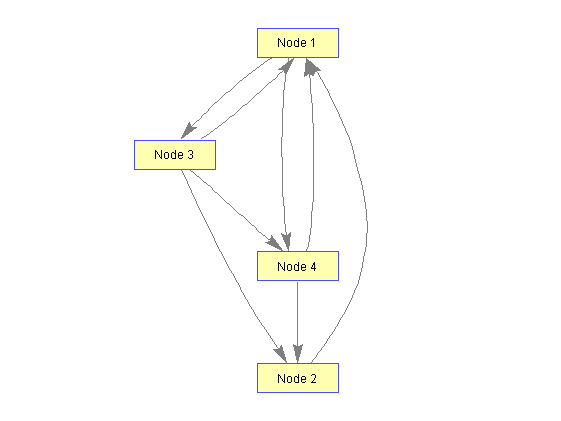
\includegraphics[scale=0.45]{../images/a1_graph.png}\label{fig:a1_graph}
	\caption{Graphe de $A_1$}
\end{figure}
\paragraph{2)} Avant de calculer la matrice de transition, il est nécessaire de caractériser la marche aléatoire. Autrement dit, il faut définir les poids/probabilités que nous appliquerons aux arêtes du graphe sur lequel le surfeur va évoluer. Nous avons déduit de l'énoncé du projet que les différentes possibilités de quitter un nœud devaient être \textbf{équiprobables} et nous utiliserons donc cette hypothèse dans la suite du rapport.
\paragraph{}
Suite à ce choix, la formation de la matrice de transition est très simple. Si l'on note $A$ la matrice d'adjacence, alors il suffit d'appliquer la formule suivante pour calculer l'élément Q(i,j) :
\[
Q(i,j) = A(i,j) \times \frac{1}{n}\sum\limits_{j = 1}^n A(i,j)
\]
Cette formule permet de placer à $0$ les éléments de $Q$ représentant une transition impossible et de placer à une certaine probabilité les autres éléments de $Q$ (toute probabilité non nulle d'une ligne de Q étant équiprobable comme attendu). Nous avons représenté le diagramme d'états à la Figure \ref{fig:Q1}

\begin{figure}[h]
	\center
	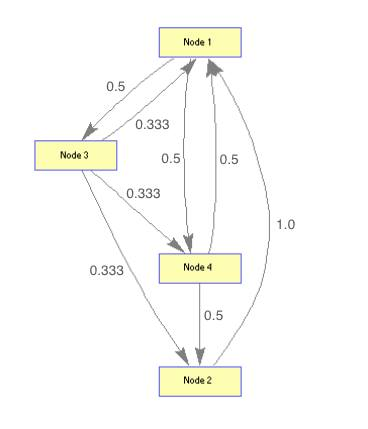
\includegraphics[scale=0.45]{../images/Q1.jpg}\label{fig:Q1}
	\caption{Diagramme d'états à partir de $A_1$}
\end{figure}

\paragraph{3)} Nous avons choisi un nombre de pas $t = 20$. Le cas où le surfeur démarre aléatoirement sur le graphe est représenté par une distribution initiale $\pi_0$ uniforme et le cas où il démarre d'une page fixe est représenté par une distribution initiale $\pi_0$ où toutes les probabilités sont nulles sauf celle située l'index correspondant au nœud de départ. L'évolution des probabilités dans les deux cas est donnée sur le Figure \ref{fig:q113}.
\begin{figure}[h]
	\center
	\subfigure{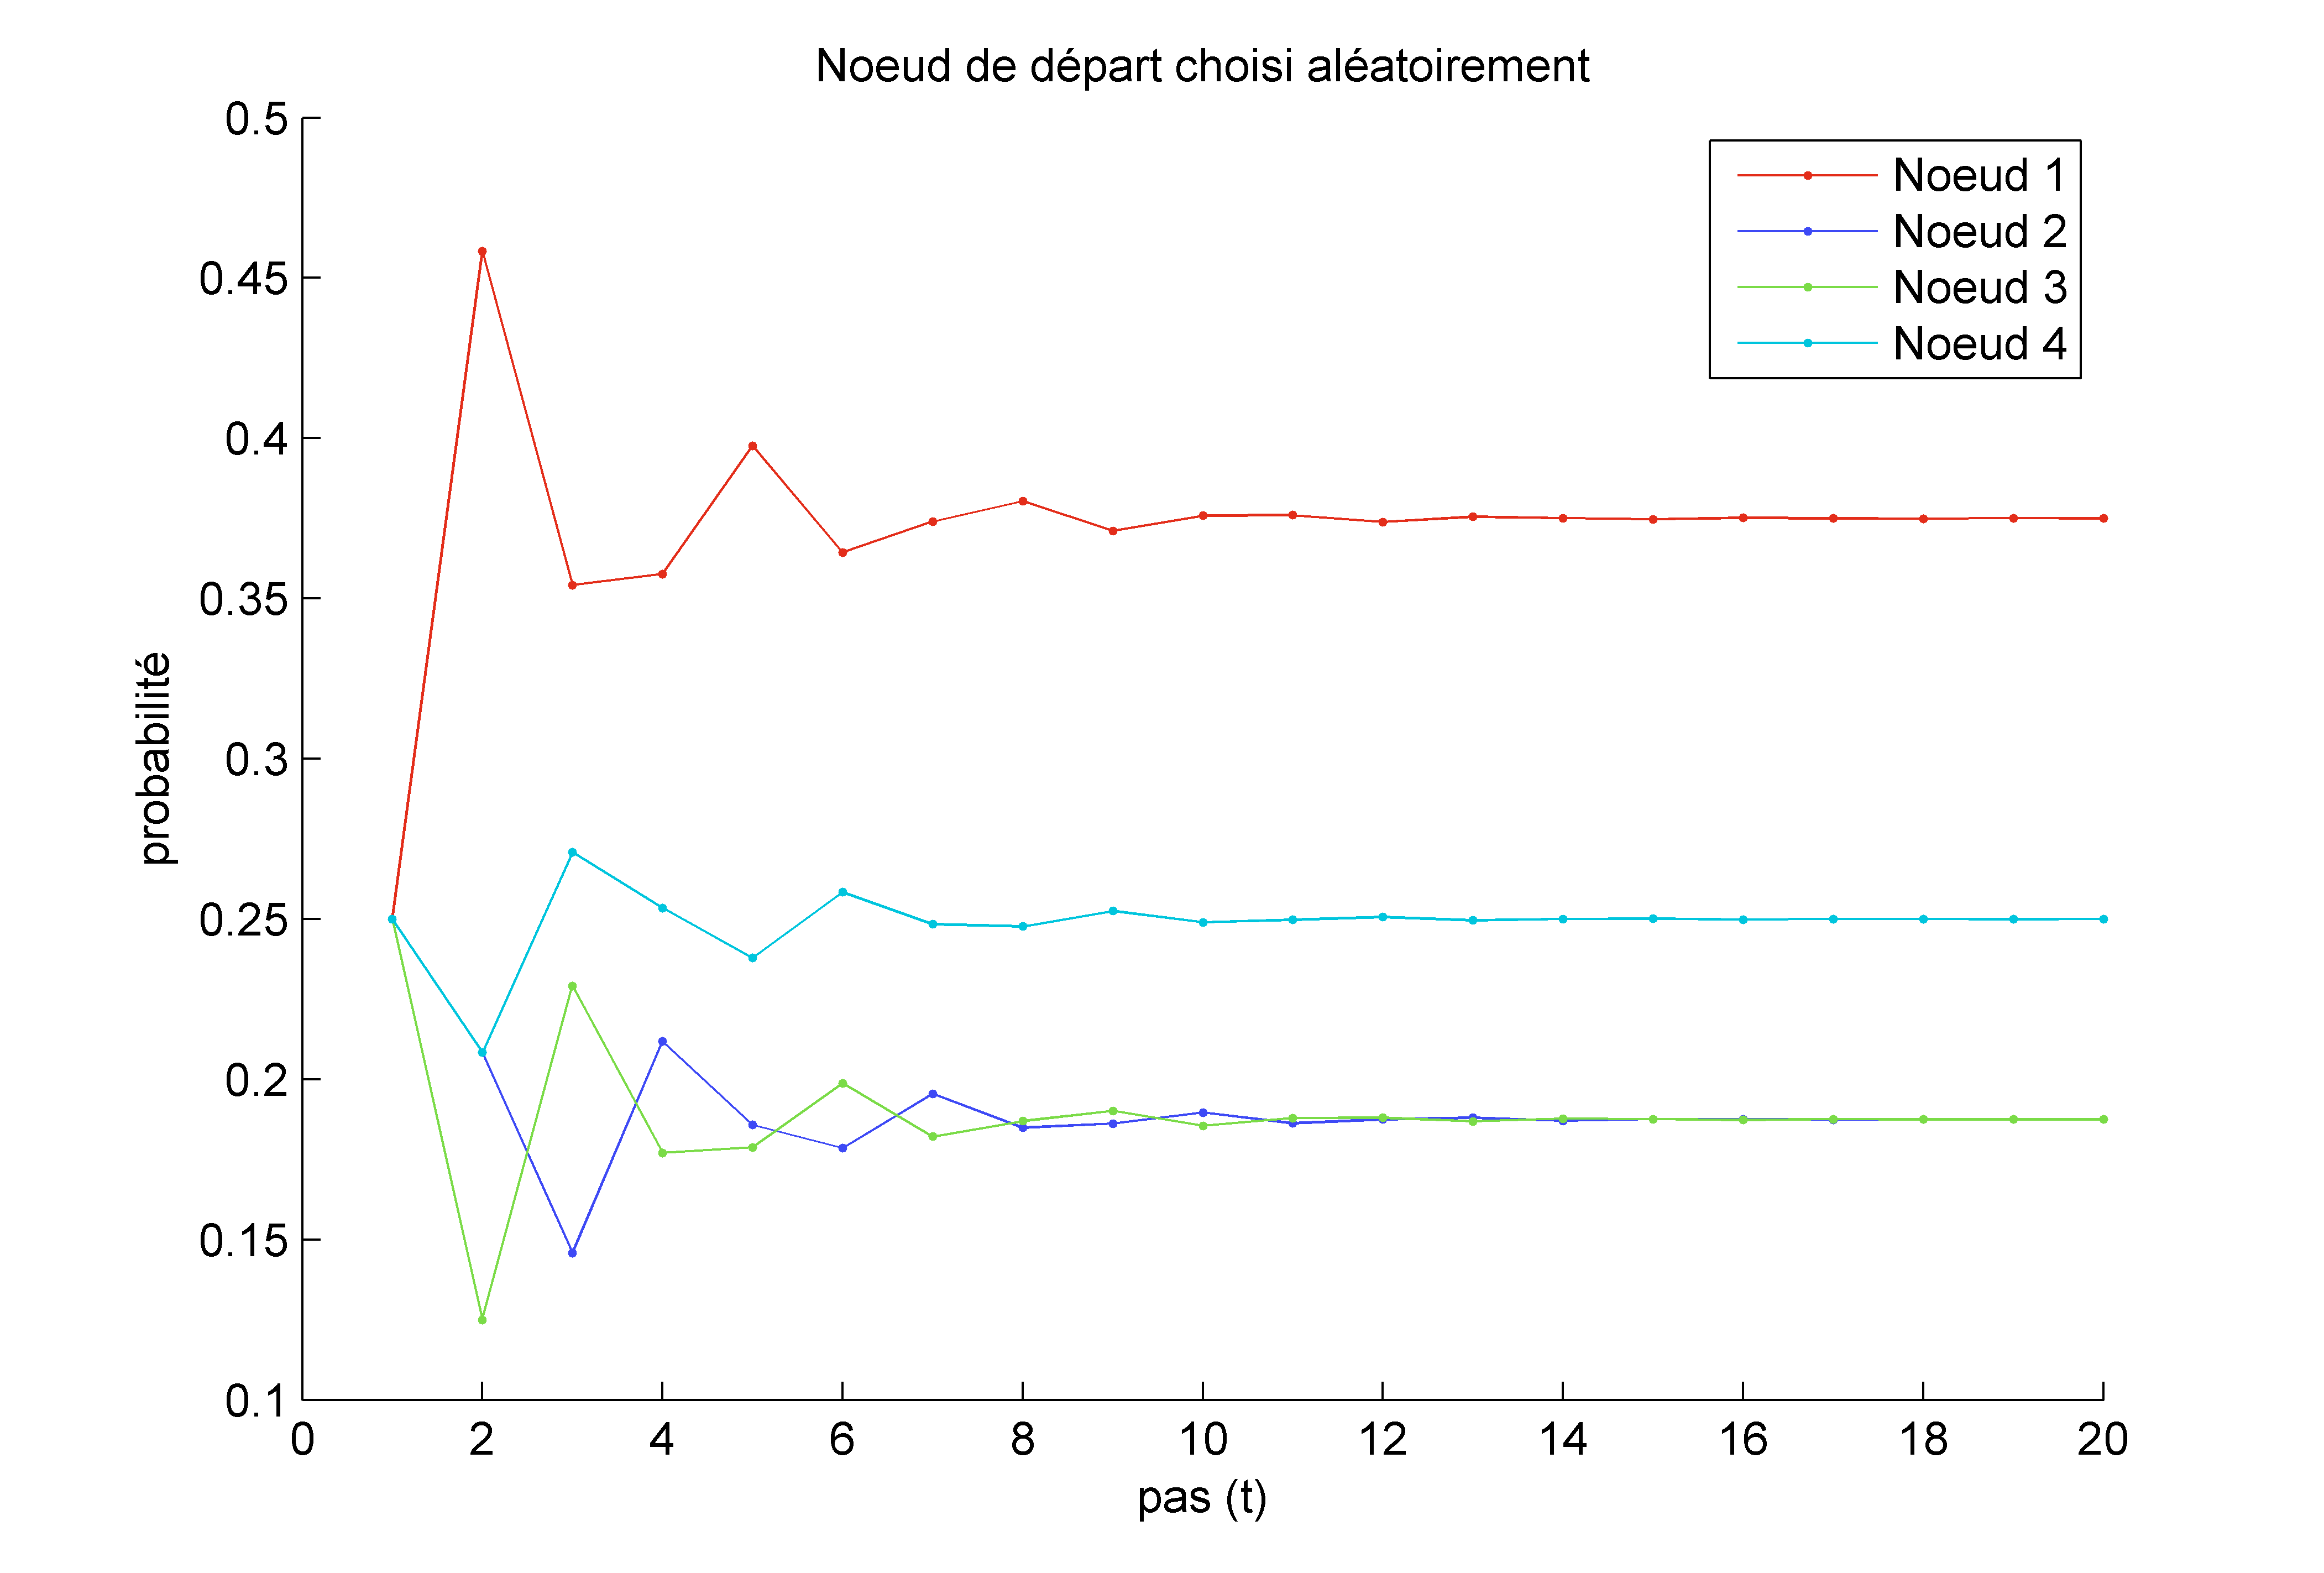
\includegraphics[scale=0.35]{../images/q1131_proba.png}}
	\subfigure{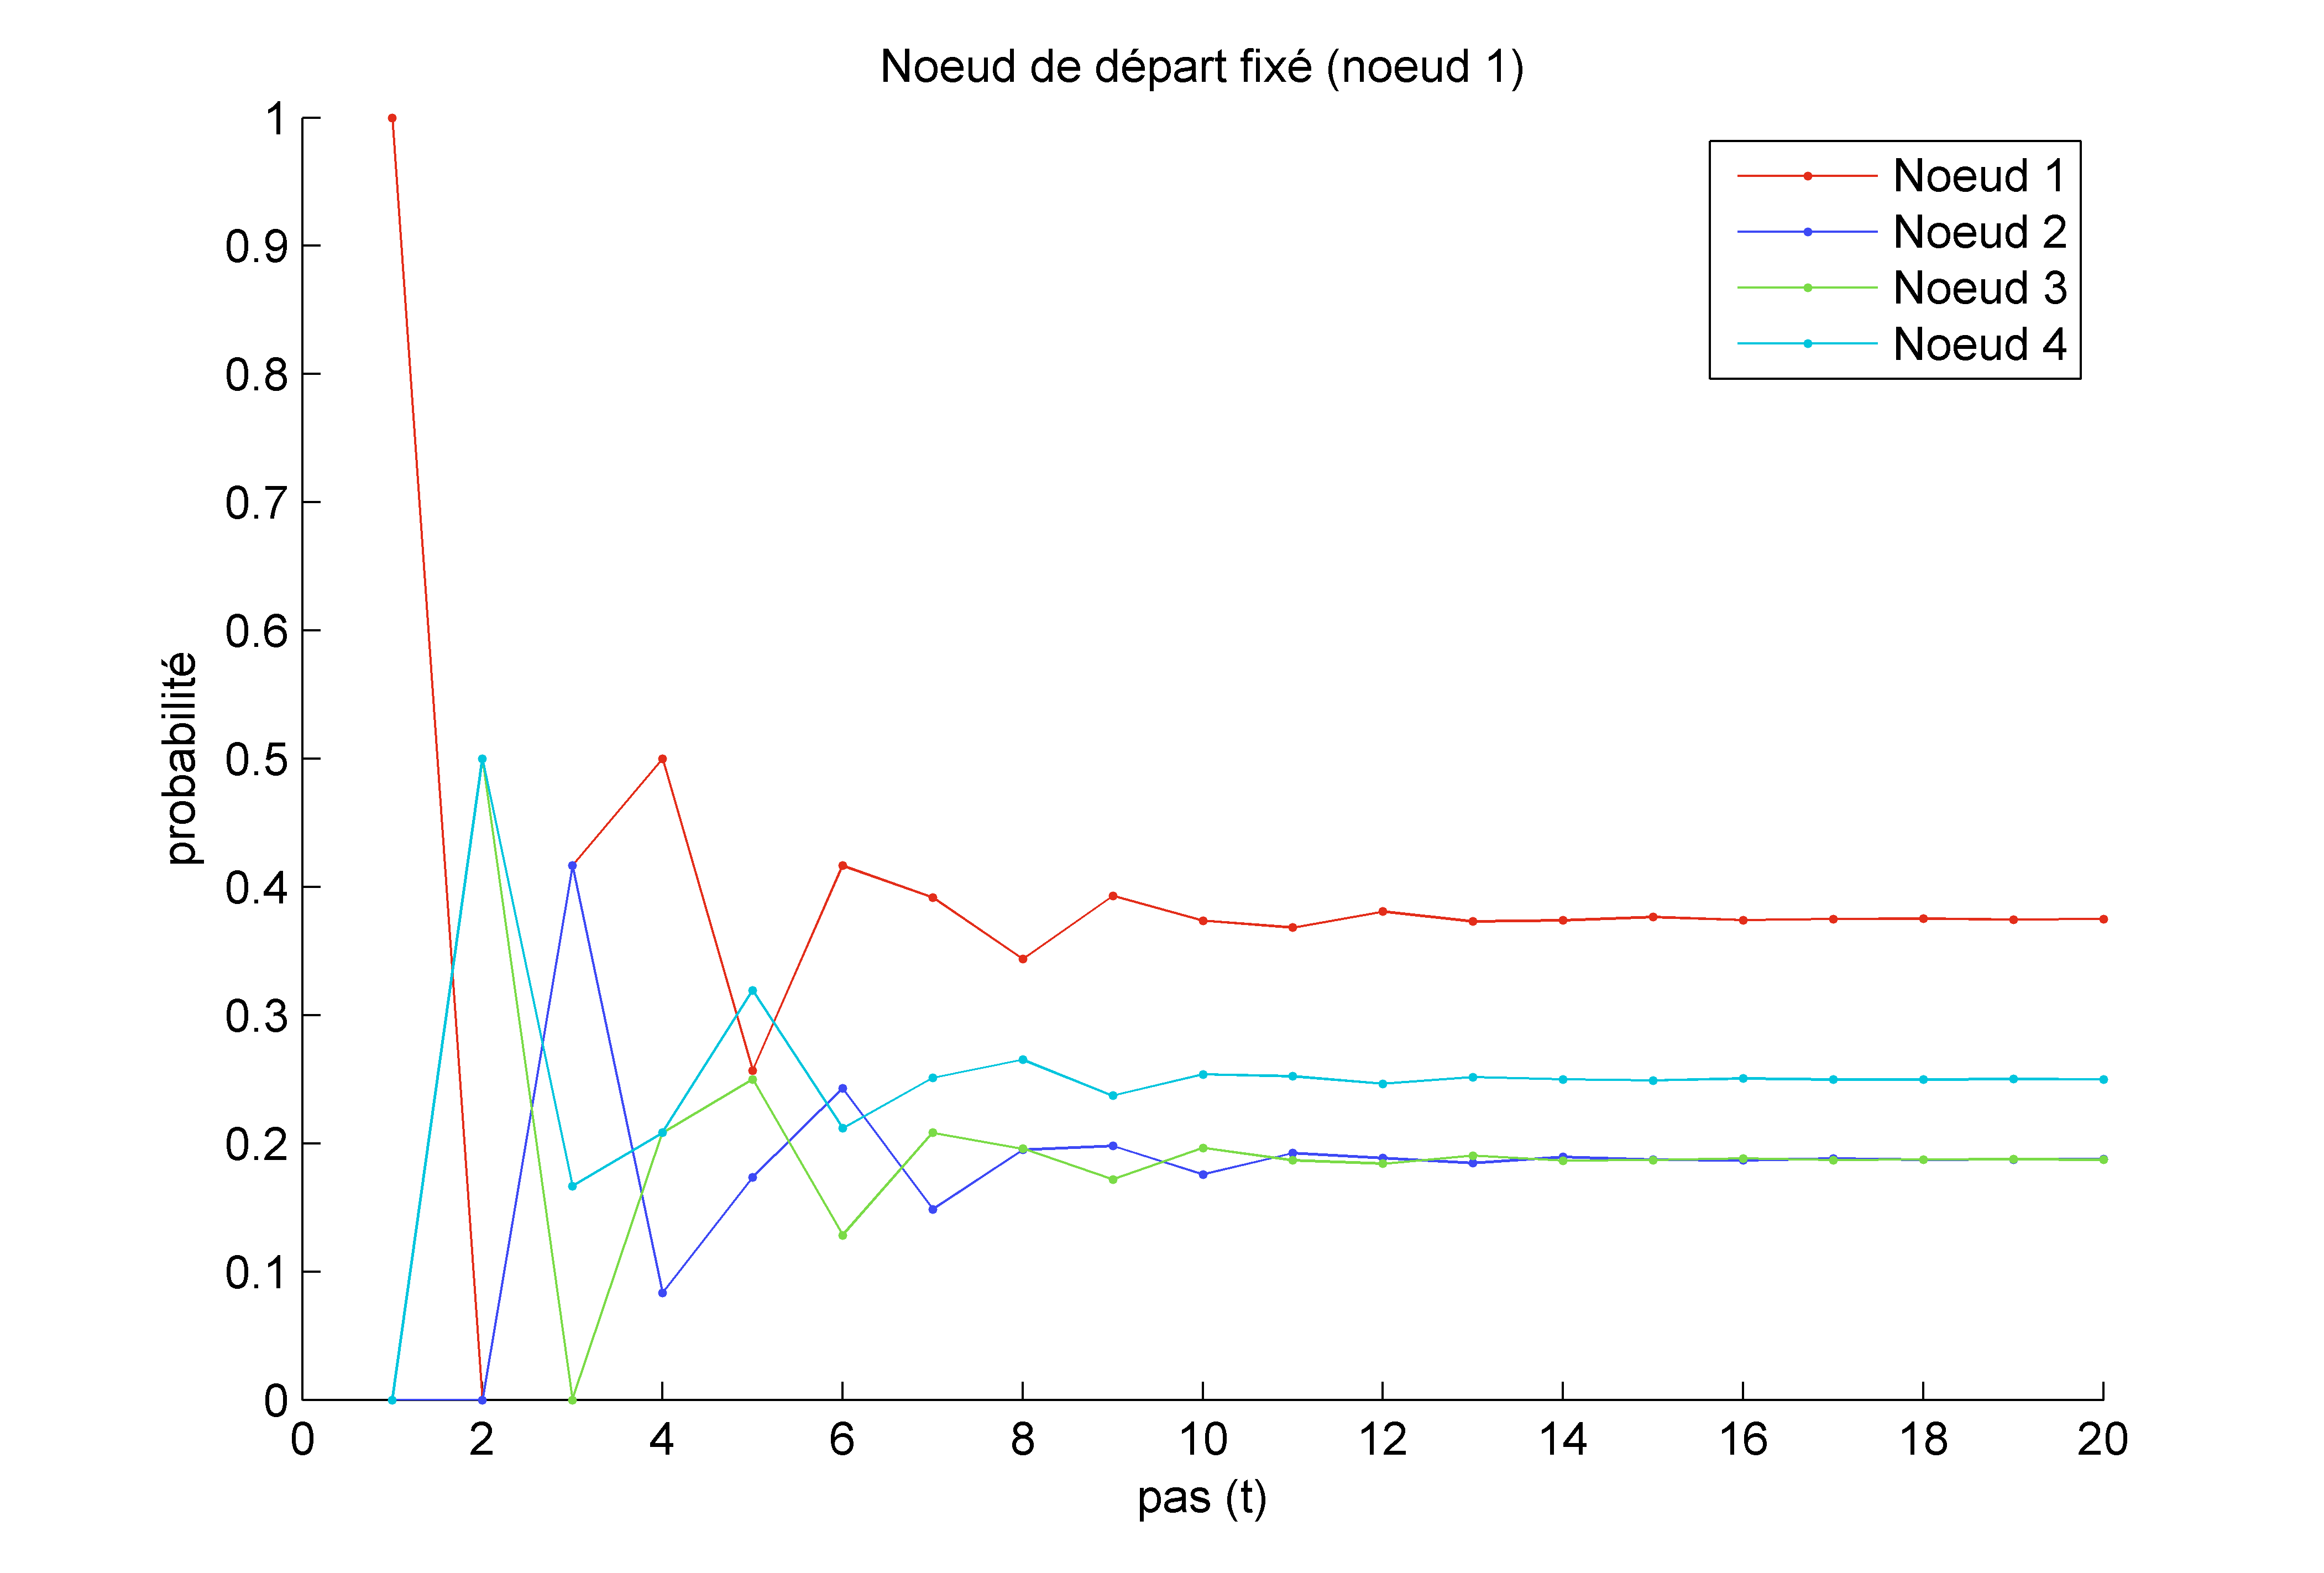
\includegraphics[scale=0.35]{../images/q1132_proba.png}}
	\caption{Évolution de la distribution de probabilité}
	\label{fig:q113}
\end{figure}
\paragraph{}
La matrice $Q^{(20)}$ obtenue est la suivante :
\[
Q^{(20)} = 
\begin{pmatrix}
 0.3751 & 0.1874 & 0.1875 & 0.2500\\
 0.3751 & 0.1877 & 0.1874 & 0.2499\\
 0.3749 & 0.1875 & 0.1875 & 0.2500\\
 0.3749 & 0.1875 & 0.1875 & 0.2500\\
\end{pmatrix}
\]
Si on observe les matrices $Q^{(k)}$ pour $k> 20$, on peut constater que les éléments se stabilisent et que les lignes s'égalisent. 
\paragraph{4)} La distribution stationnaire a été calculée par la méthode des puissances. Nous avons donc multiplié les distributions $\pi^{(k)}$ successives par $Q$ jusqu'à ce que cette distribution se stabilise. Le critère de stabilisation choisi était le suivant : 
\[
\max\left(\left|\pi_j^{(k)} - \pi_j^{(k - 1)}\pi\right|\right) < \varepsilon
\]
où $\pi_j$ est la $j^{\text{ième}}$ composante du vecteur $\pi$. La distribution stationnaire obtenue est donnée ci-dessous :
\[
\pi_\infty = 
\begin{pmatrix}
0.3750 &
0.1875 &
0.1875 &
0.2500 \\
\end{pmatrix}
\]
On constate que les lignes de la matrice sont très proches des valeurs observables sur les graphiques du point précédent.
\paragraph{5)} On constate que le noeud 1 possède le meilleur PageRank, suivi des noeuds 2 et 3 à égalité et du noeud 4. On peut expliquer ce classement intuitivement : 
\begin{itemize}
	\item le \textbf{noeud 1} possède le plus d'arêtes entrantes donc ayant le plus de chance d'être visité
	\item le \textbf{noeud 3} possède le moins d'arêtes entrantes donc ayant le moins de chance d'être visité
	\item les \textbf{noeuds 2} et \textbf{4} possèdent le même nombre intermédiaire (par rapport aux deux autres) d'arêtes entrantes. Le PageRank du noeud 4 est néanmoins plus élevé que celui du noeud 2 puisque le noeud 4 possèdent une arête entrante venant du noeud 1 qui est le plus visité.
	\item malgré un nombre d'arêtes entrantes plus élevé que pour le noeud 3, le \textbf{noeud 2} possède une PageRank égal. Cela est dû au fait que, d'une part, le noeud 3 peut être visité depuis le noeud le plus visité (noeud 1) ce qui améliore son PageRank et, d'autre part, que le noeud 2 ne peut être accédé depuis des noeuds moins visités (noeud 3 et 4) ce qui abaisse son PageRank. 
\end{itemize} 
\paragraph{6)} Dans un premier temps, nous avons généré une chaîne pour chaque longueur. Le résultat obtenu est donné sur la Figure \ref{sfig:q116_evol_1}. On peut déjà observer que les différentes courbes obtenues oscillent autour de leur probabilité stationnaire correspondante. Néanmoins, étant donné la présence d'oscillations, nous avons décidé de refaire l'expérience en générant cette fois-ci 1000 chaînes pour chaque longueur. Nous avons ensuite moyenné les différentes probabilités afin d'obtenir un résultat plus précis (voir Figure \ref{sfig:q116_evol_2}). Les courbes obtenues nous permettent de confirmer les premières observations.
\paragraph{}
Remarquons aussi que, quelque soit la distribution de départ, la distribution converge vers la distribution stationnaire.
\begin{figure}[h]
	\center
	\subfigure[1 génération]{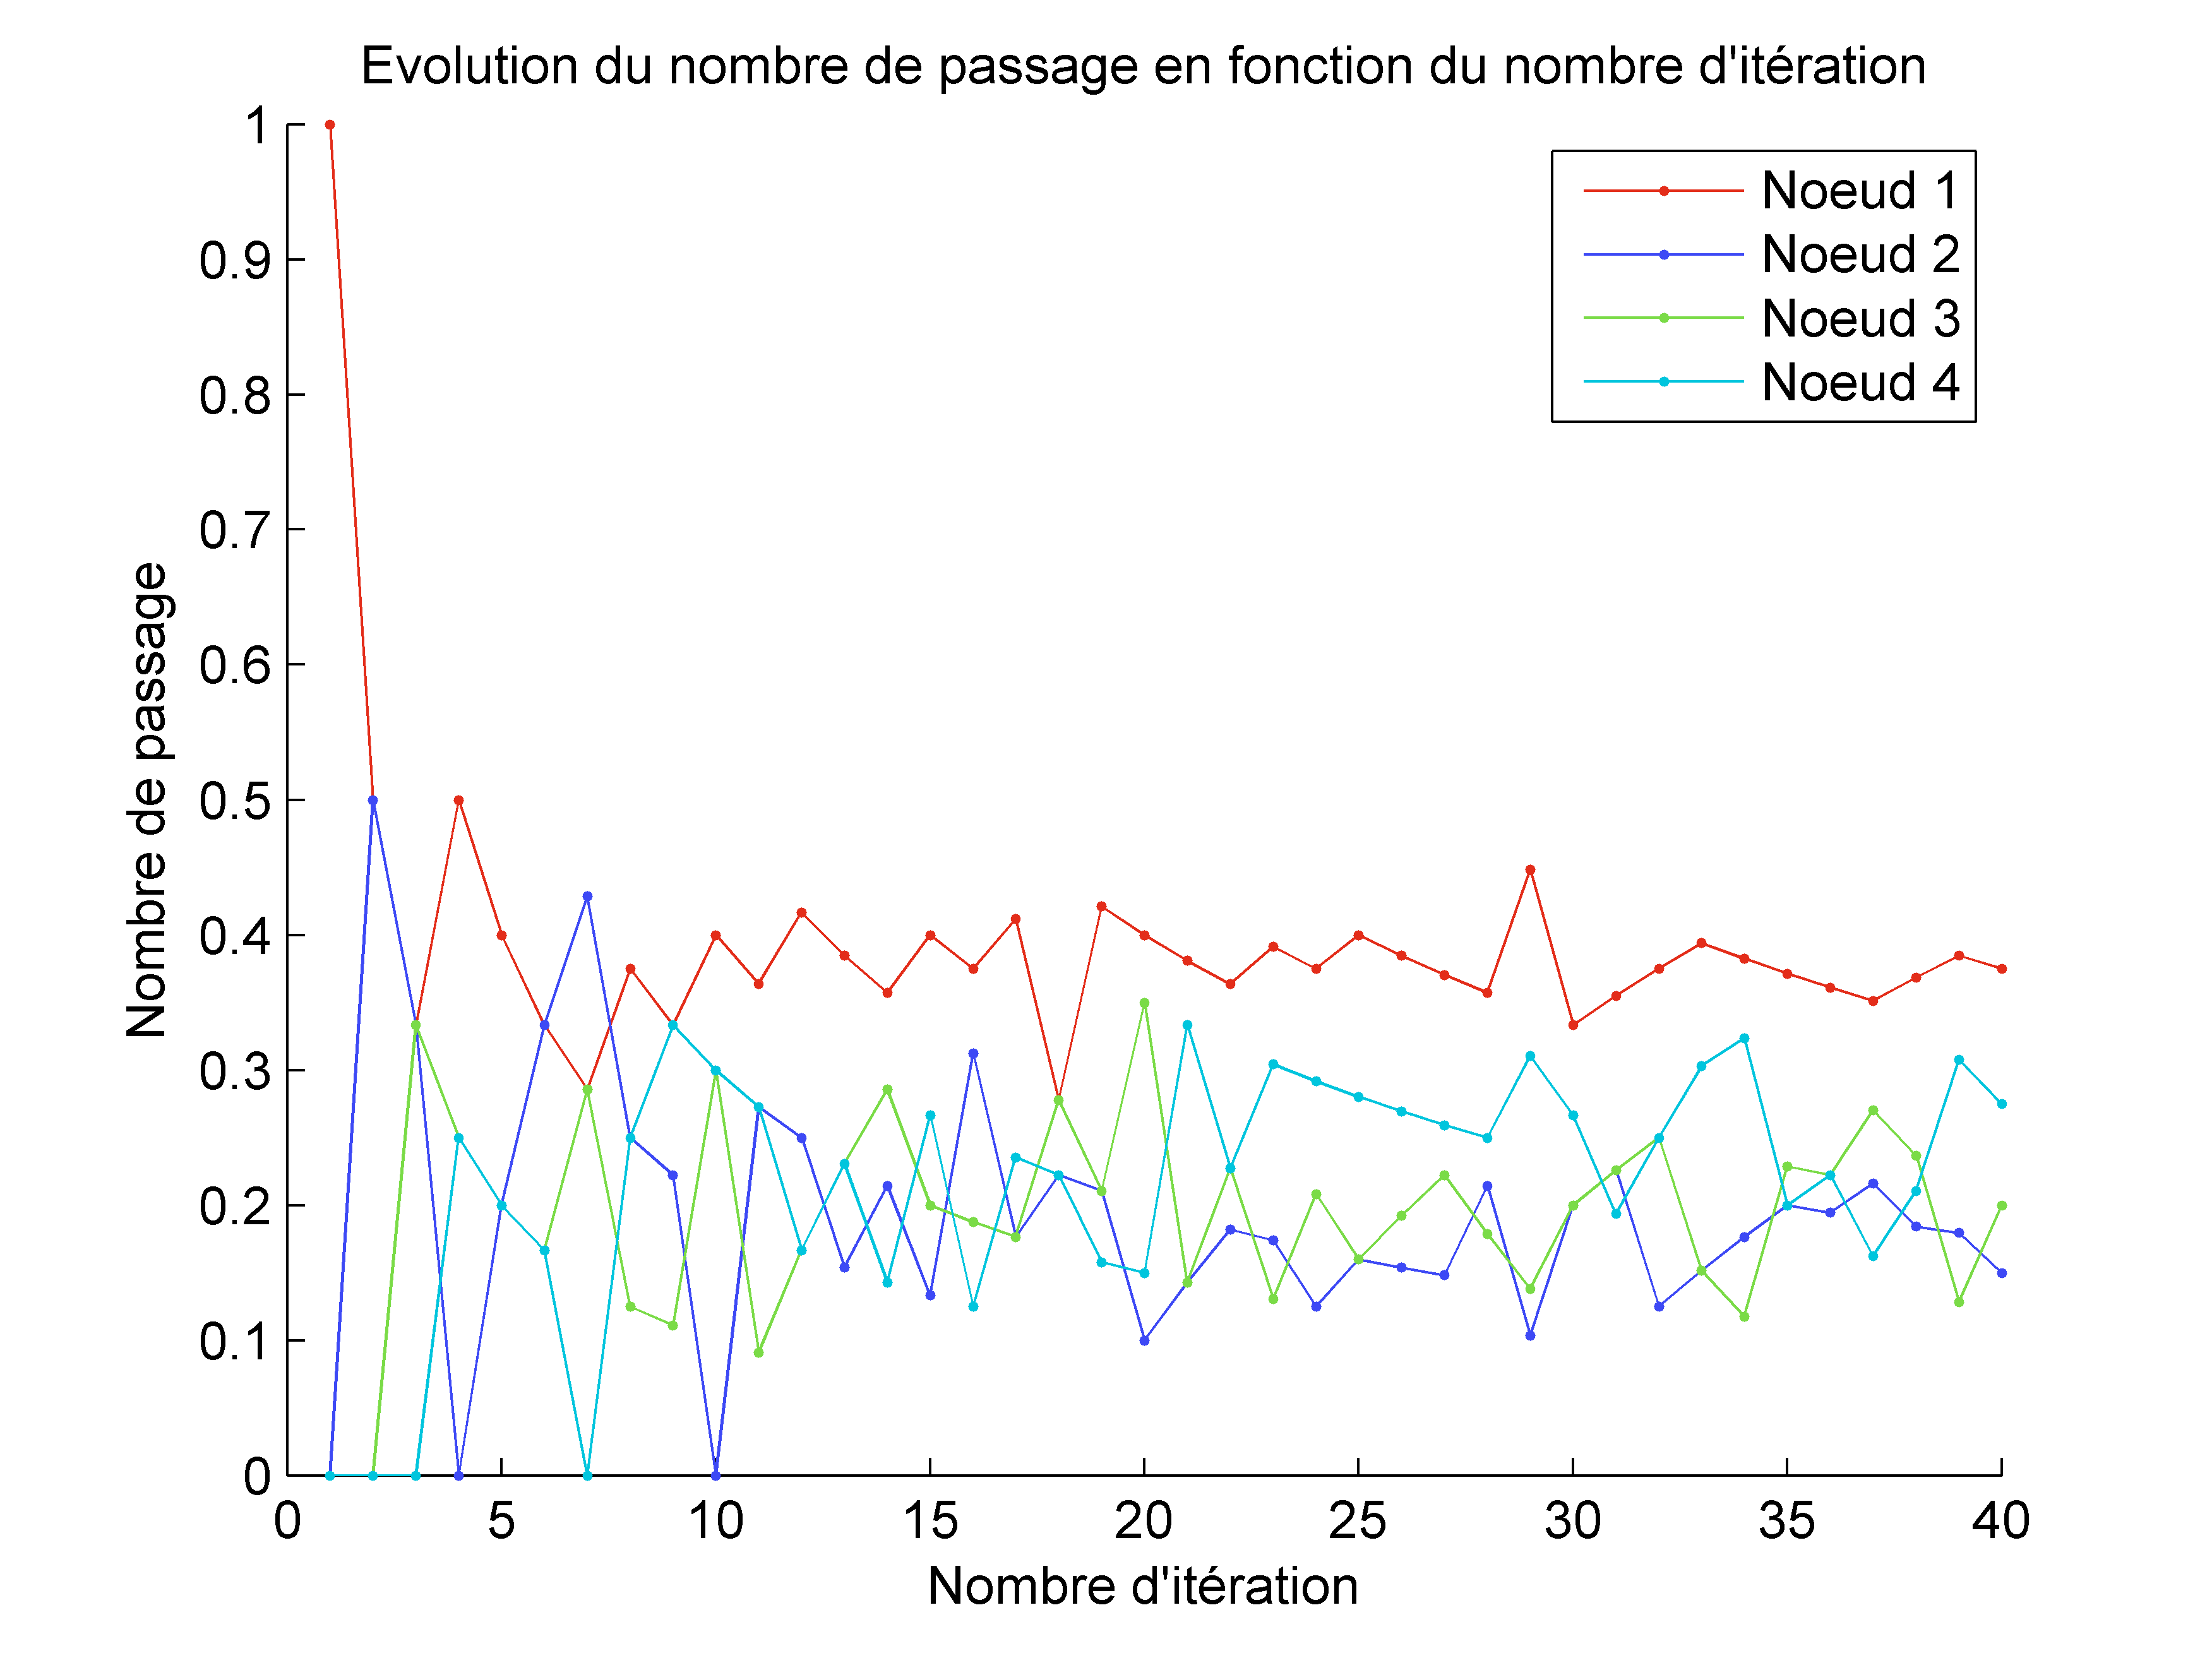
\includegraphics[scale=0.45]{../images/q116_evol_1.png}\label{sfig:q116_evol_1}}
	\subfigure[1000 générations]{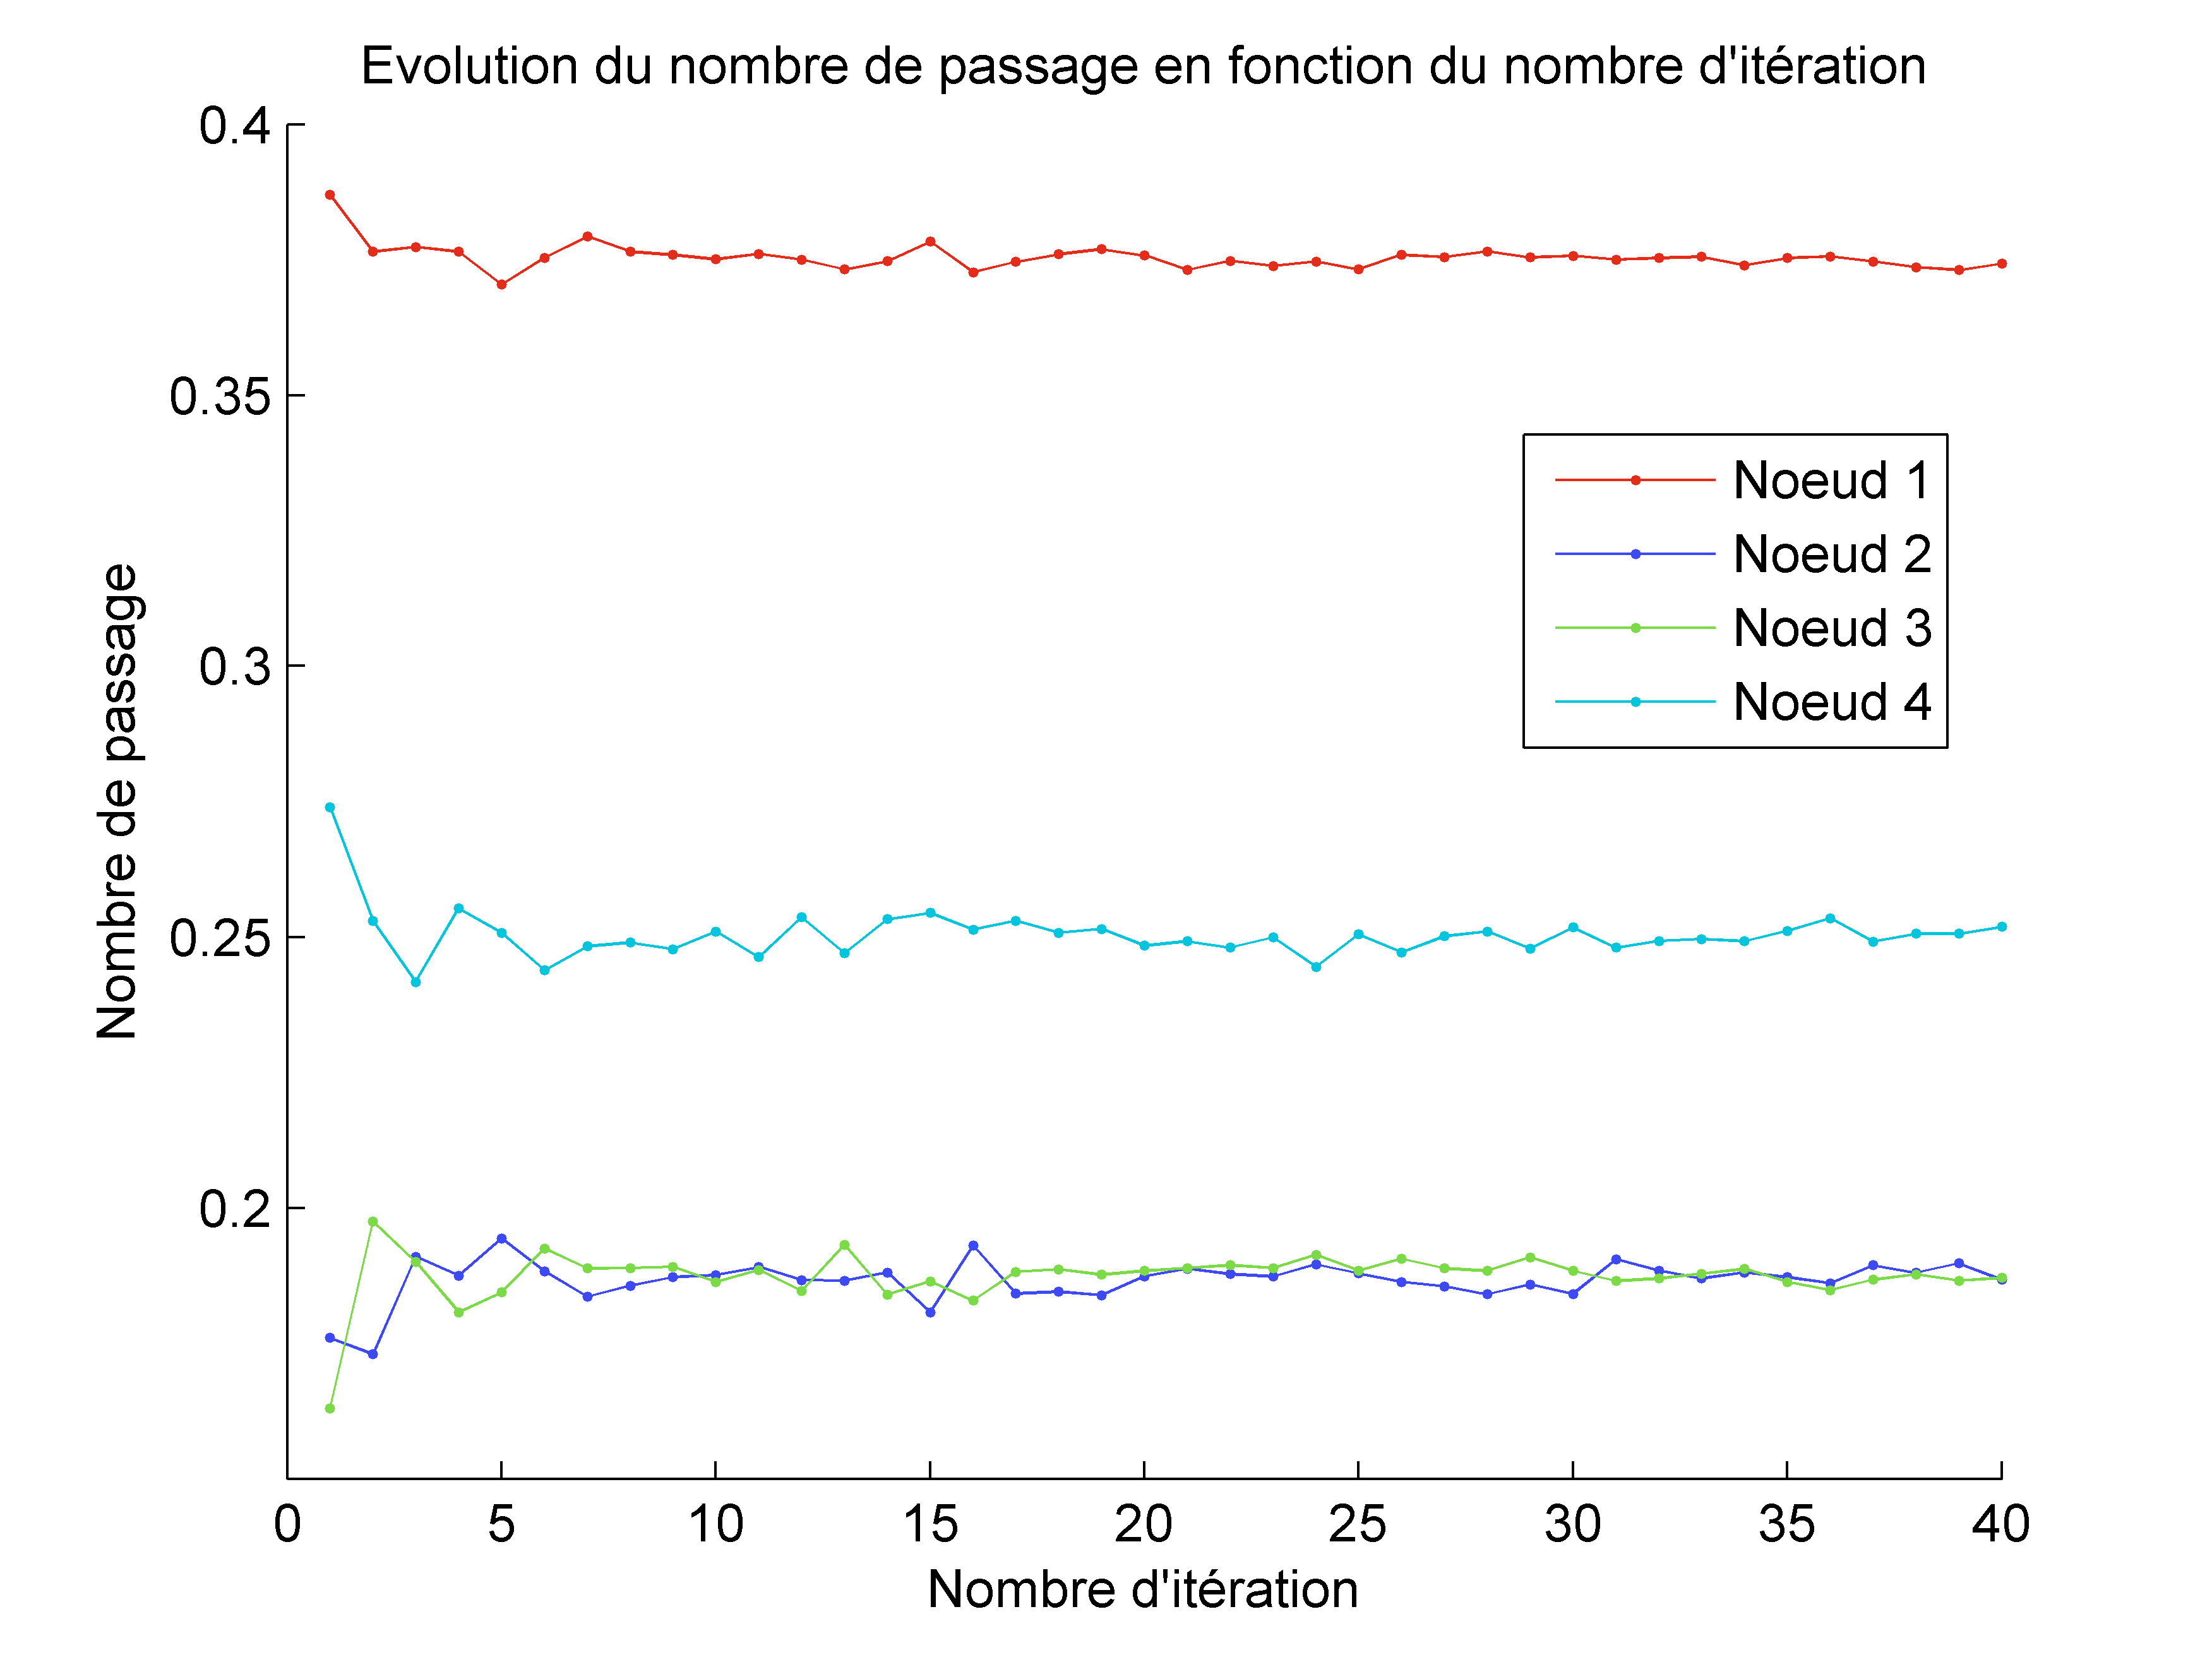
\includegraphics[scale=0.45]{../images/q116_evol_2.png}\label{sfig:q116_evol_2}}
	\caption{Évolution du nombre de passage par un noeud}
\end{figure}
\paragraph{7)} 
Nous pouvons relier ces résultats à la théorie car la chaîne est \textbf{\textit{ergodique}}. En effet : \\
\begin{itemize}
\item[•] Premièrement, la chaîne est \textbf{\textit{irréductible}} car il est possible de visiter tous les autres noeuds à partir de n'importe quel noeud donné.
\item[•] Deuxièmement, la chaîne est \textbf{\textit{apériodique}} car le plus grand commun diviseur du nombre de pas nécessaires \textbf{N} pour aller d'un noeud vers lui même est inférieur à 2. Si on analyse le graphe, on observe que pour les noeuds 1, 3 et 4 le nombre de pas nécessaires vaut 2 alors que ce nombre vaut trois pour le noeud 2. \textbf{N} vaut donc 1.\\
\end{itemize}

Dans l'expérience du point 6, nous avons observé que la distribution de probabilité stationnaire correspond aux probabilités trouvées sur nos graphes lorsque le nombre d'itérations est assez élevé .


\subsection{Analyse des matrices $A_2$ et $A_3$}
\paragraph{1)} Pour pouvoir calculer des éventuelles distributions stationnaires sur base des matrices $A_2$ et $A_3$, nous avons calculé les matrices de transition $Q_2$ et $Q_3$ : 
\[
Q_2 = 
\begin{pmatrix}
         0 &   1.0000  &       0  &       0 \\
         0 &        0  &       0  &  1.0000 \\
    0.5000 &   0.5000  &       0  &       0 \\
    1.0000 &        0  &       0  &       0 \\
\end{pmatrix}
Q_3 = 
\begin{pmatrix}
        0  &   1.0000   &      0  &       0  &       0 \\
    1.0000 &        0   &      0  &       0  &       0 \\
         0 &   0.3333   &      0  &  0.3333  &  0.3333 \\
         0 &        0   &      0  &       0  &  1.0000 \\
         0 &        0   &      0  &  1.0000  &       0 \\
\end{pmatrix}
\]
Nous avons représenté les diagrammes d'états des deux chaînes de Markov sur la Figure \ref{sfig:Q23}. 
\begin{figure}[h]
	\center
	\subfigure{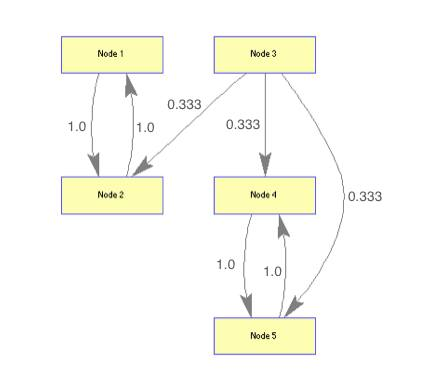
\includegraphics[scale=0.45]{../images/Q2.jpg}}
	\subfigure{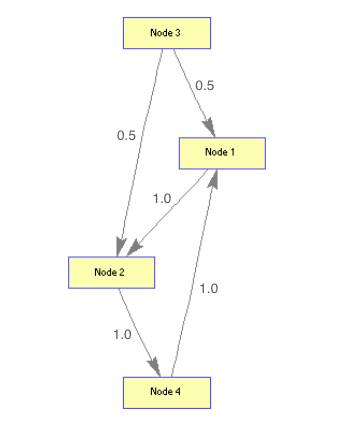
\includegraphics[scale=0.45]{../images/Q3.jpg}}
	\caption{Diagramme d'état de $A_2$ et $A_3$}
	\label{fig:Q23}
\end{figure} 
Nous avons ensuite appliqué la méthode des puissance pour obtenir des distributions $\pi^{(k)}$ successives. Le résultat est donné sur la Figure \ref{fig:q118}. On constate qu'aucune distribution stationnaire n'a pu être trouvée étant donné la présence d'\textbf{oscillations}.
\paragraph{}
On constate aussi que la \textbf{probabilité} d'atteindre une certain nœud \textbf{tombe à 0} ou est directement nulle dès la première itération dans les deux situations. Ce phénomène est dû à la présence de \textit{dangling nodes} dans les deux graphes. On peut directement voir la présence de type de nœud sur les matrices de transitions :  elle se manifeste par une colonne composée uniquement de probabilités nulles et implique qu'il est impossible de passer d'un nœud quelconque au \textit{dangling node}.
\paragraph{}
Ces deux phénomènes sont précisément des \textbf{limitations} du modèle du surfeur aléatoire simpliste présenté dans cette première partie. D'une part, les oscillations empêchent d'atteindre une distribution stationnaire. D'autre part, la probabilité nulle d'atteindre un nœud existant rend l'éventuelle distribution stationnaire (et donc le PageRank) peut représentative de l'organisation des nœuds puisqu'elle en omet d'en prendre certains en compte.
\paragraph{}
Les\textbf{ causes de ces phénomènes} sont d'une part la présence d'un cycle  infini dans les graphes et la présence de \textit{dangling nodes}. Ces problèmes vont être contournés en introduisant la téléportation dans la section suivante.
\begin{figure}[h]
	\center
	\subfigure[Distribution initiale uniforme]{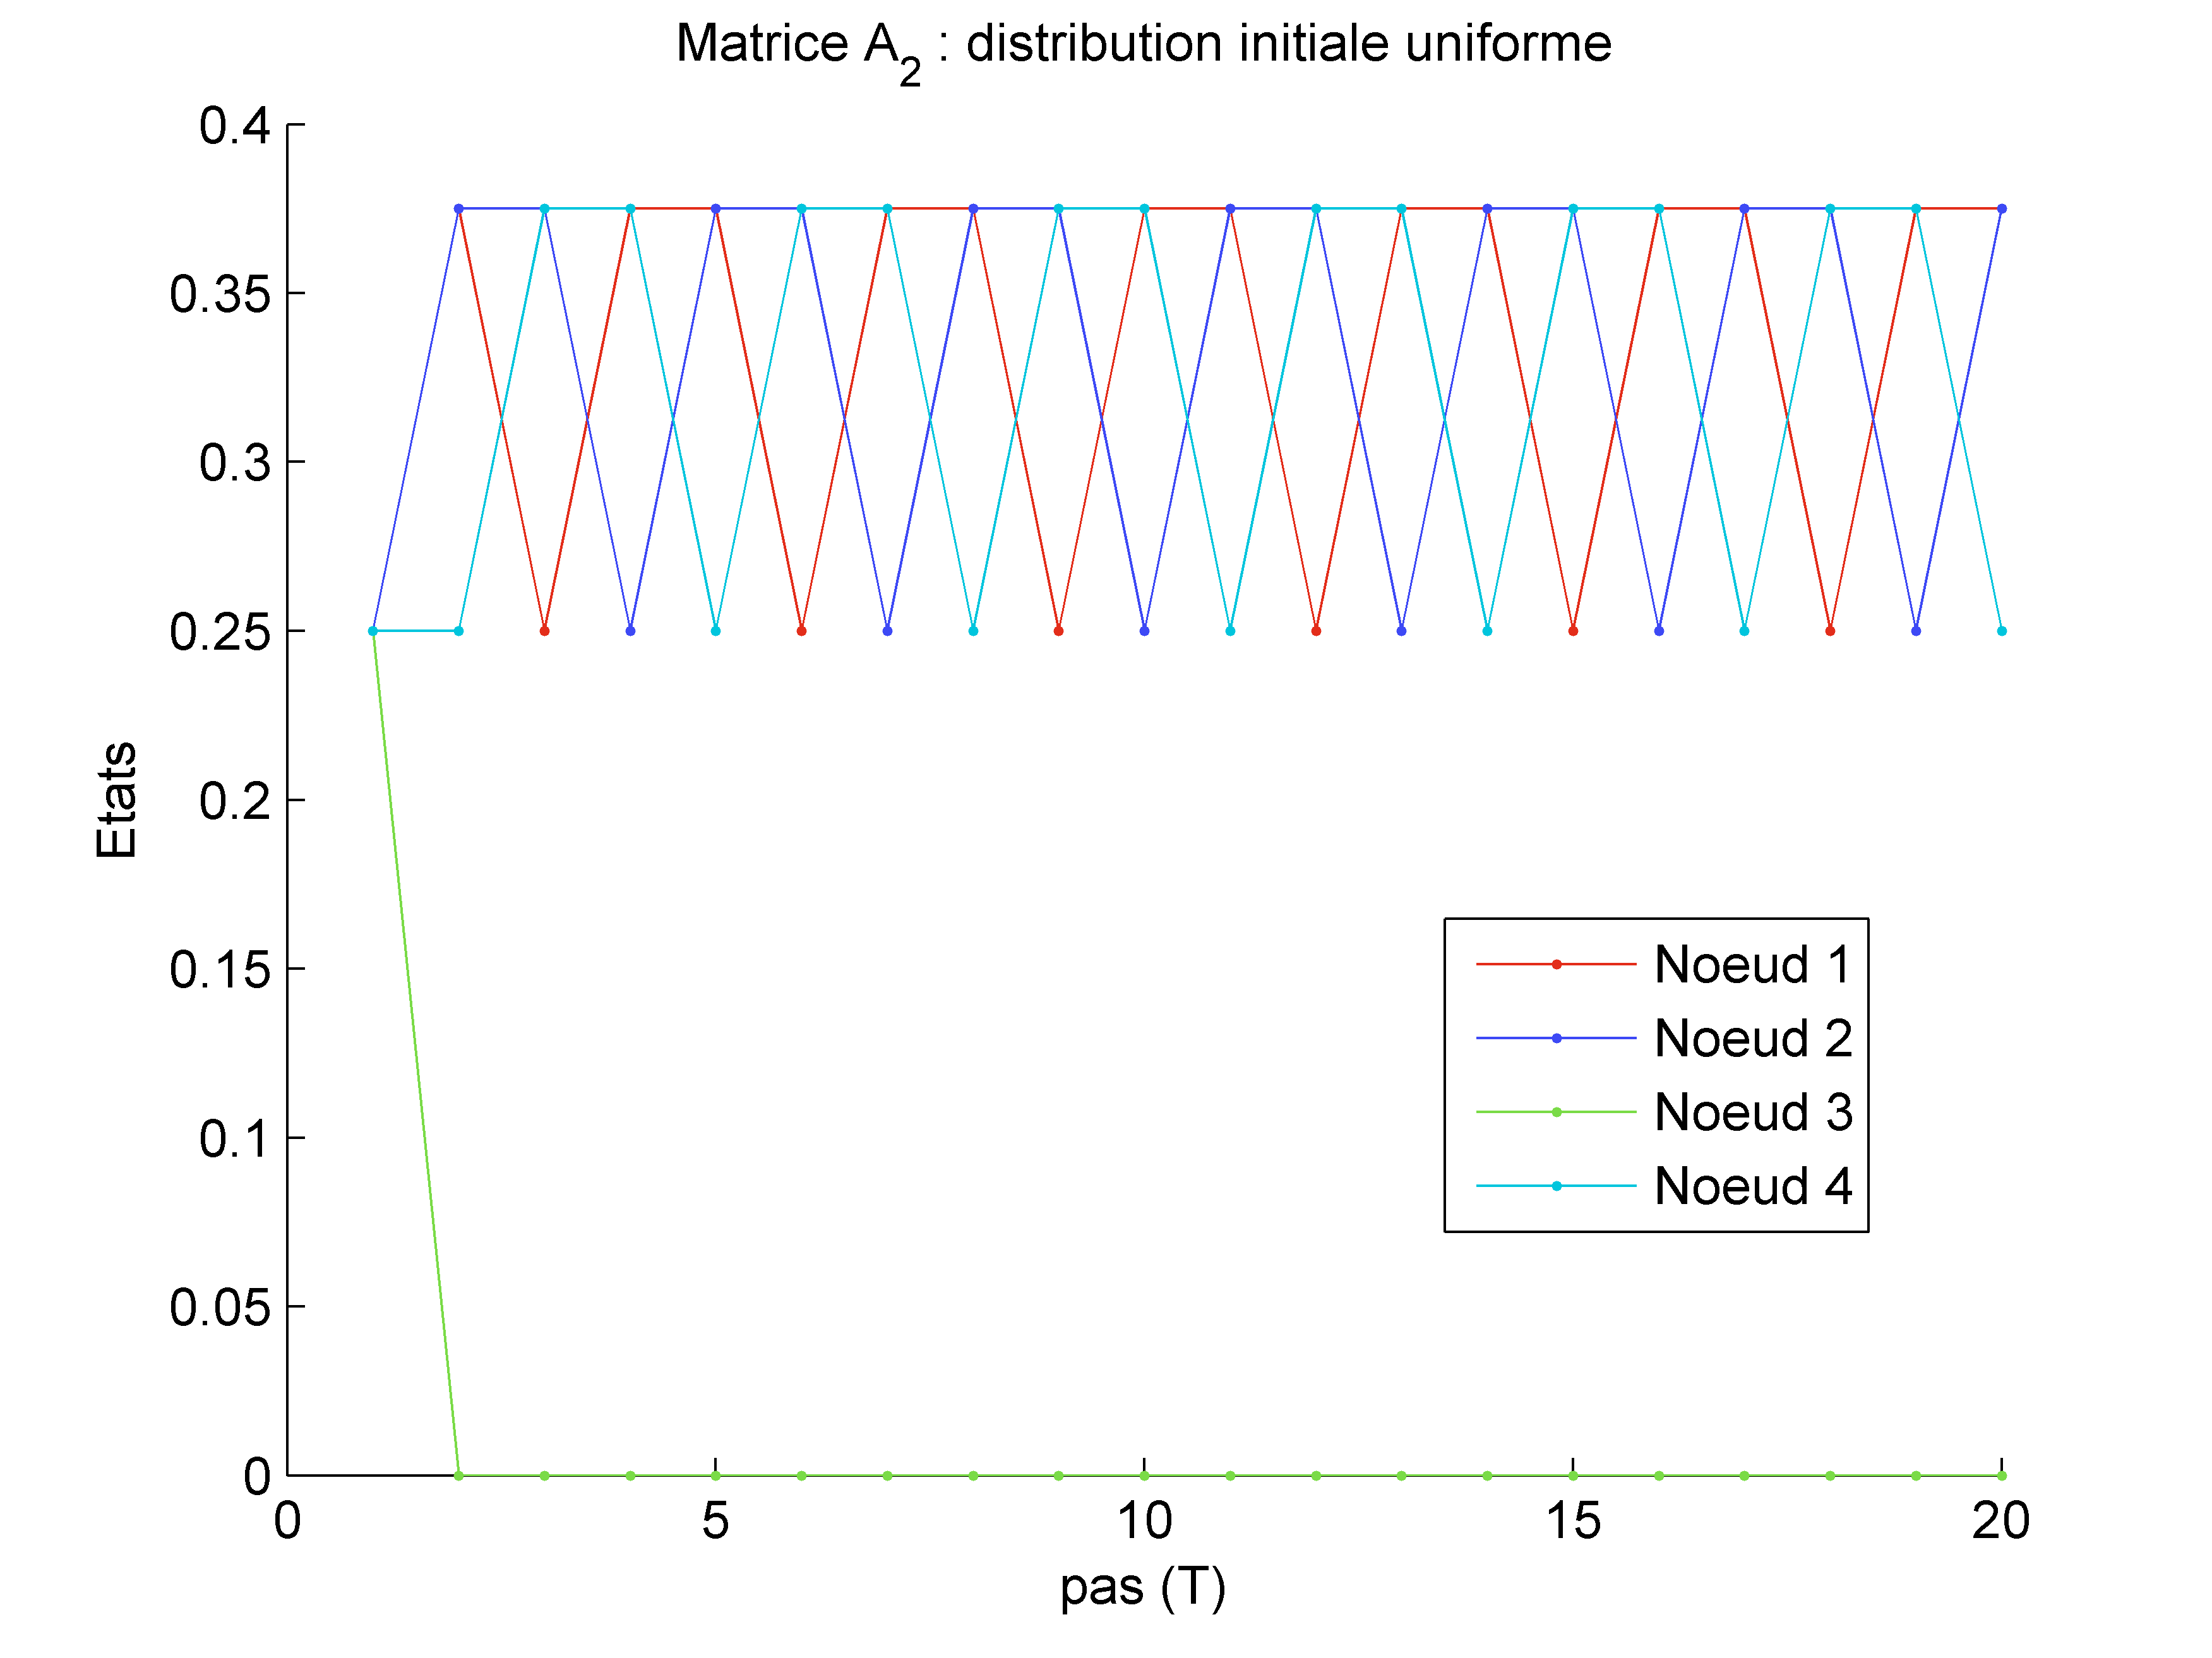
\includegraphics[scale=0.45]{../images/q118_evol_21.png}\label{sfig:q118_evol}}
	\subfigure[Depuis le noeud 1]{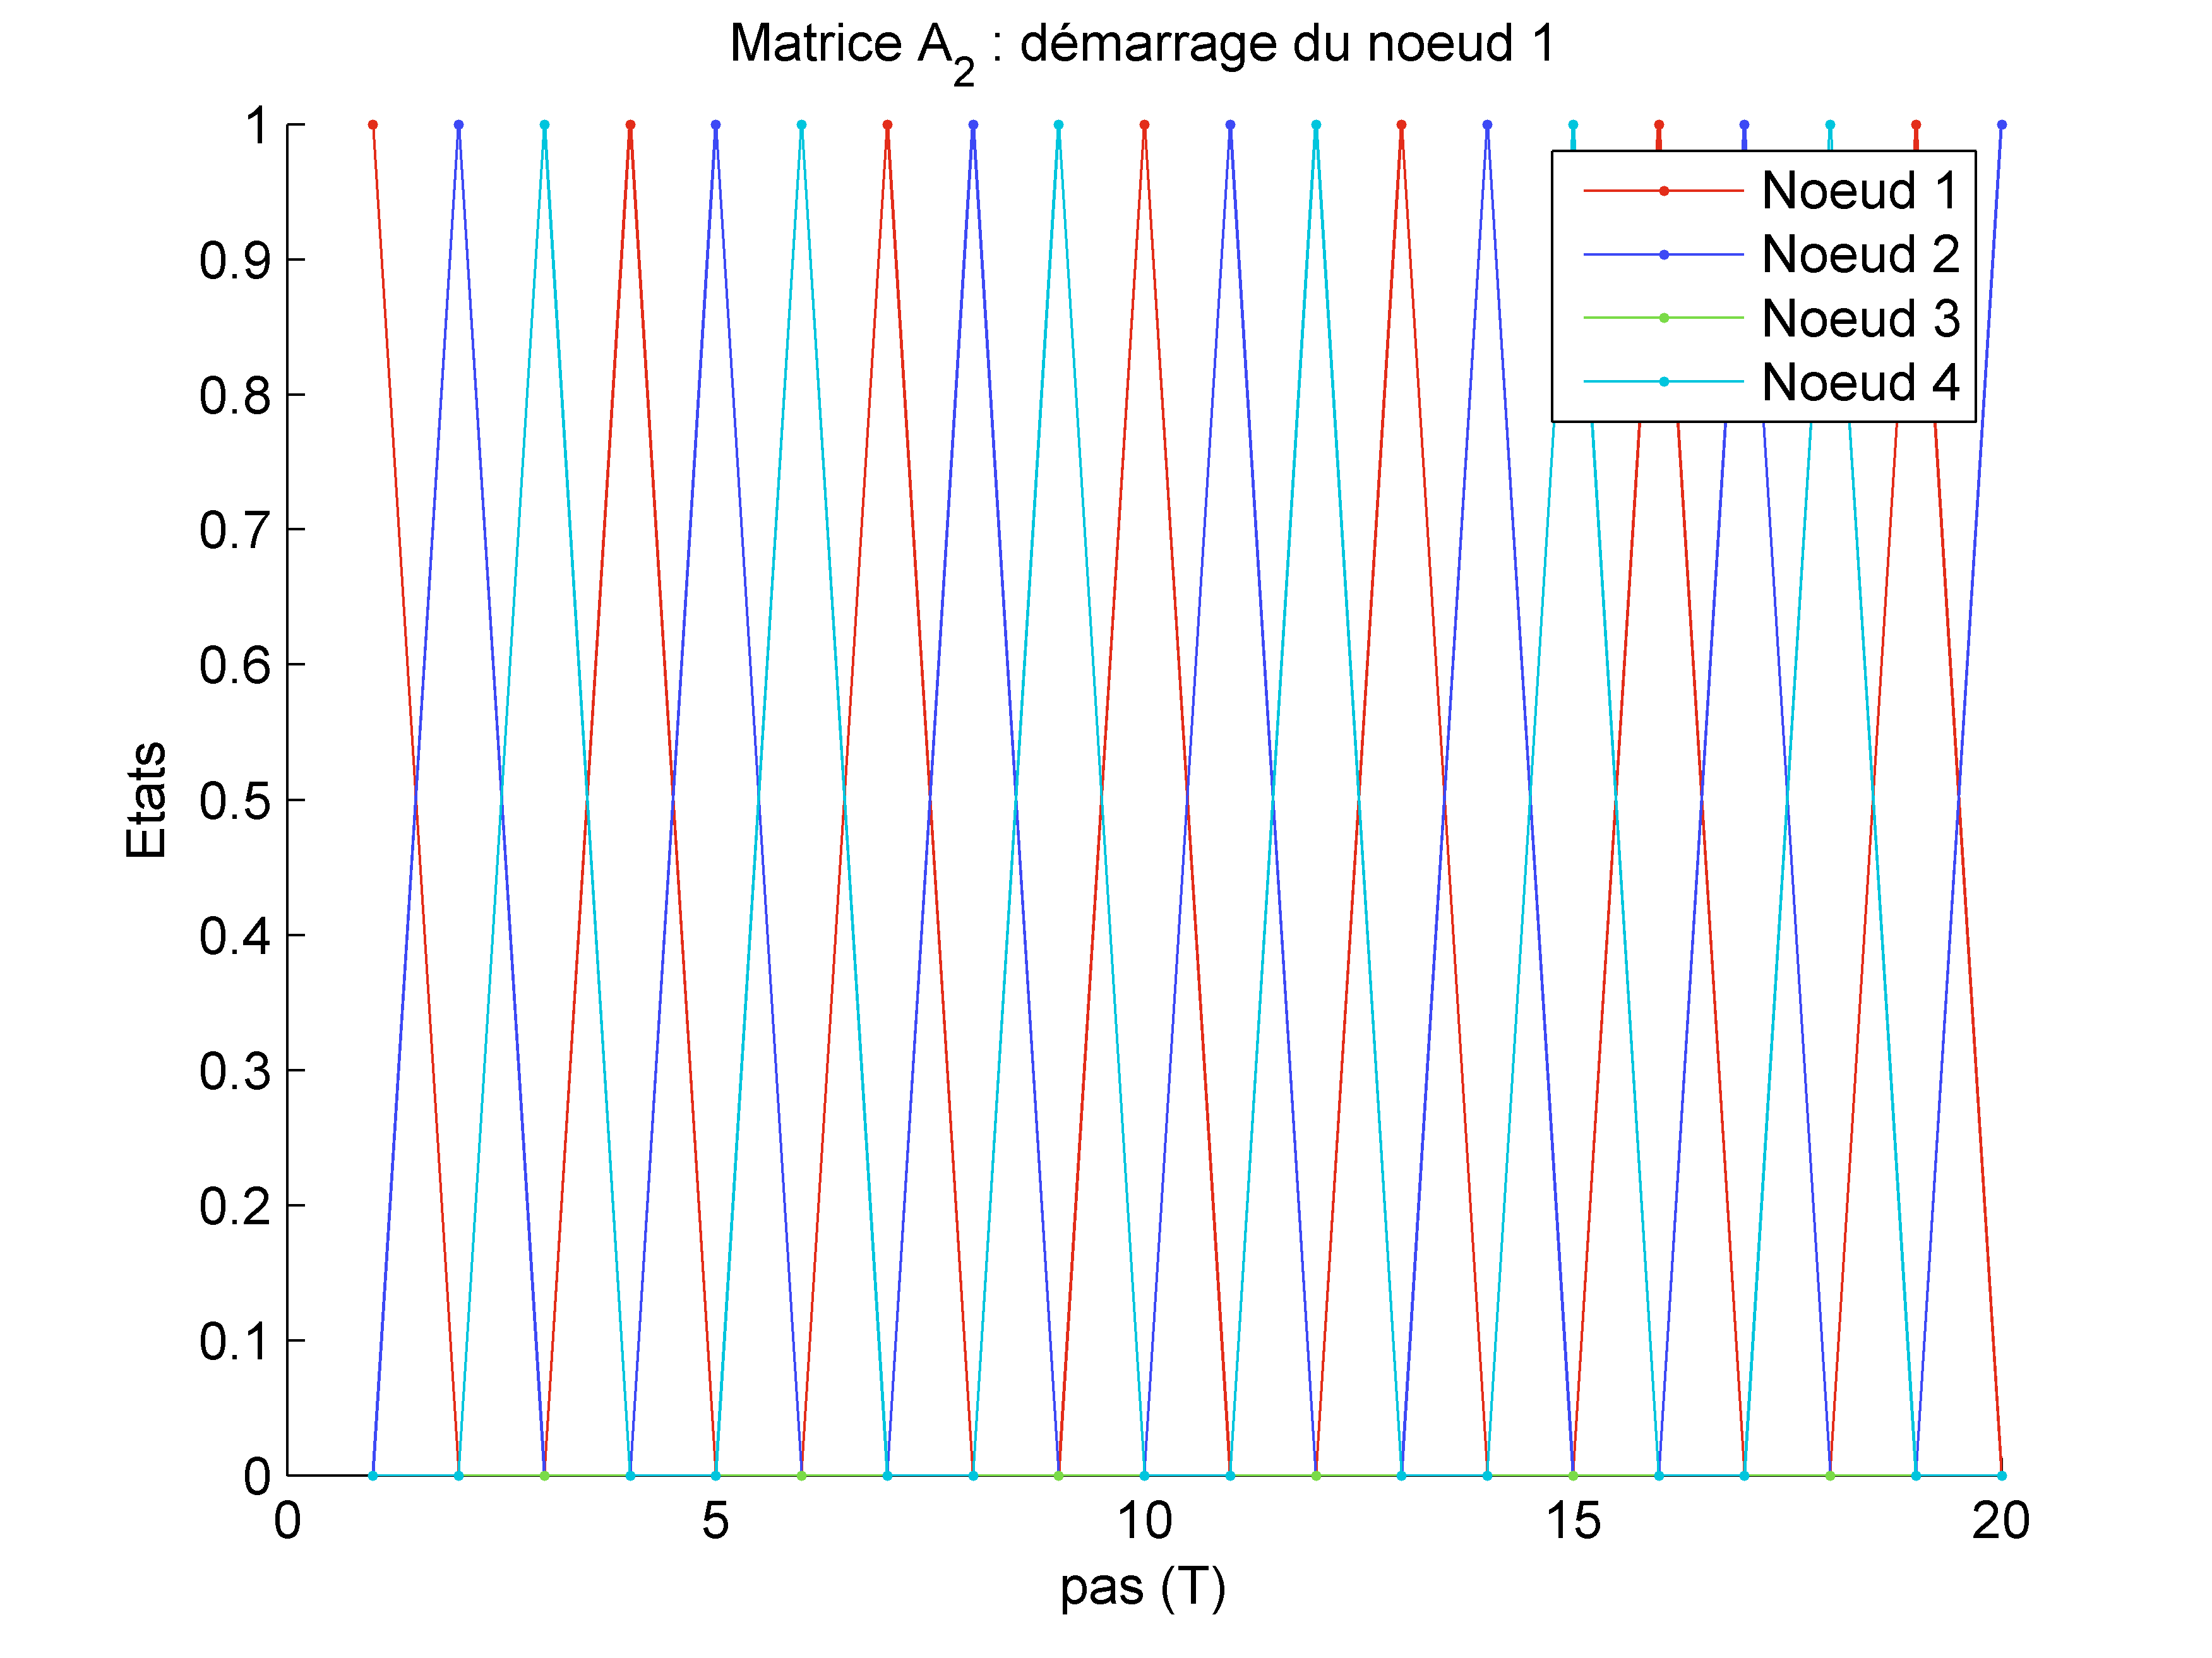
\includegraphics[scale=0.45]{../images/q118_evol_22.png}\label{sfig:q118_evol}}
	\subfigure[Distribution initiale uniforme]{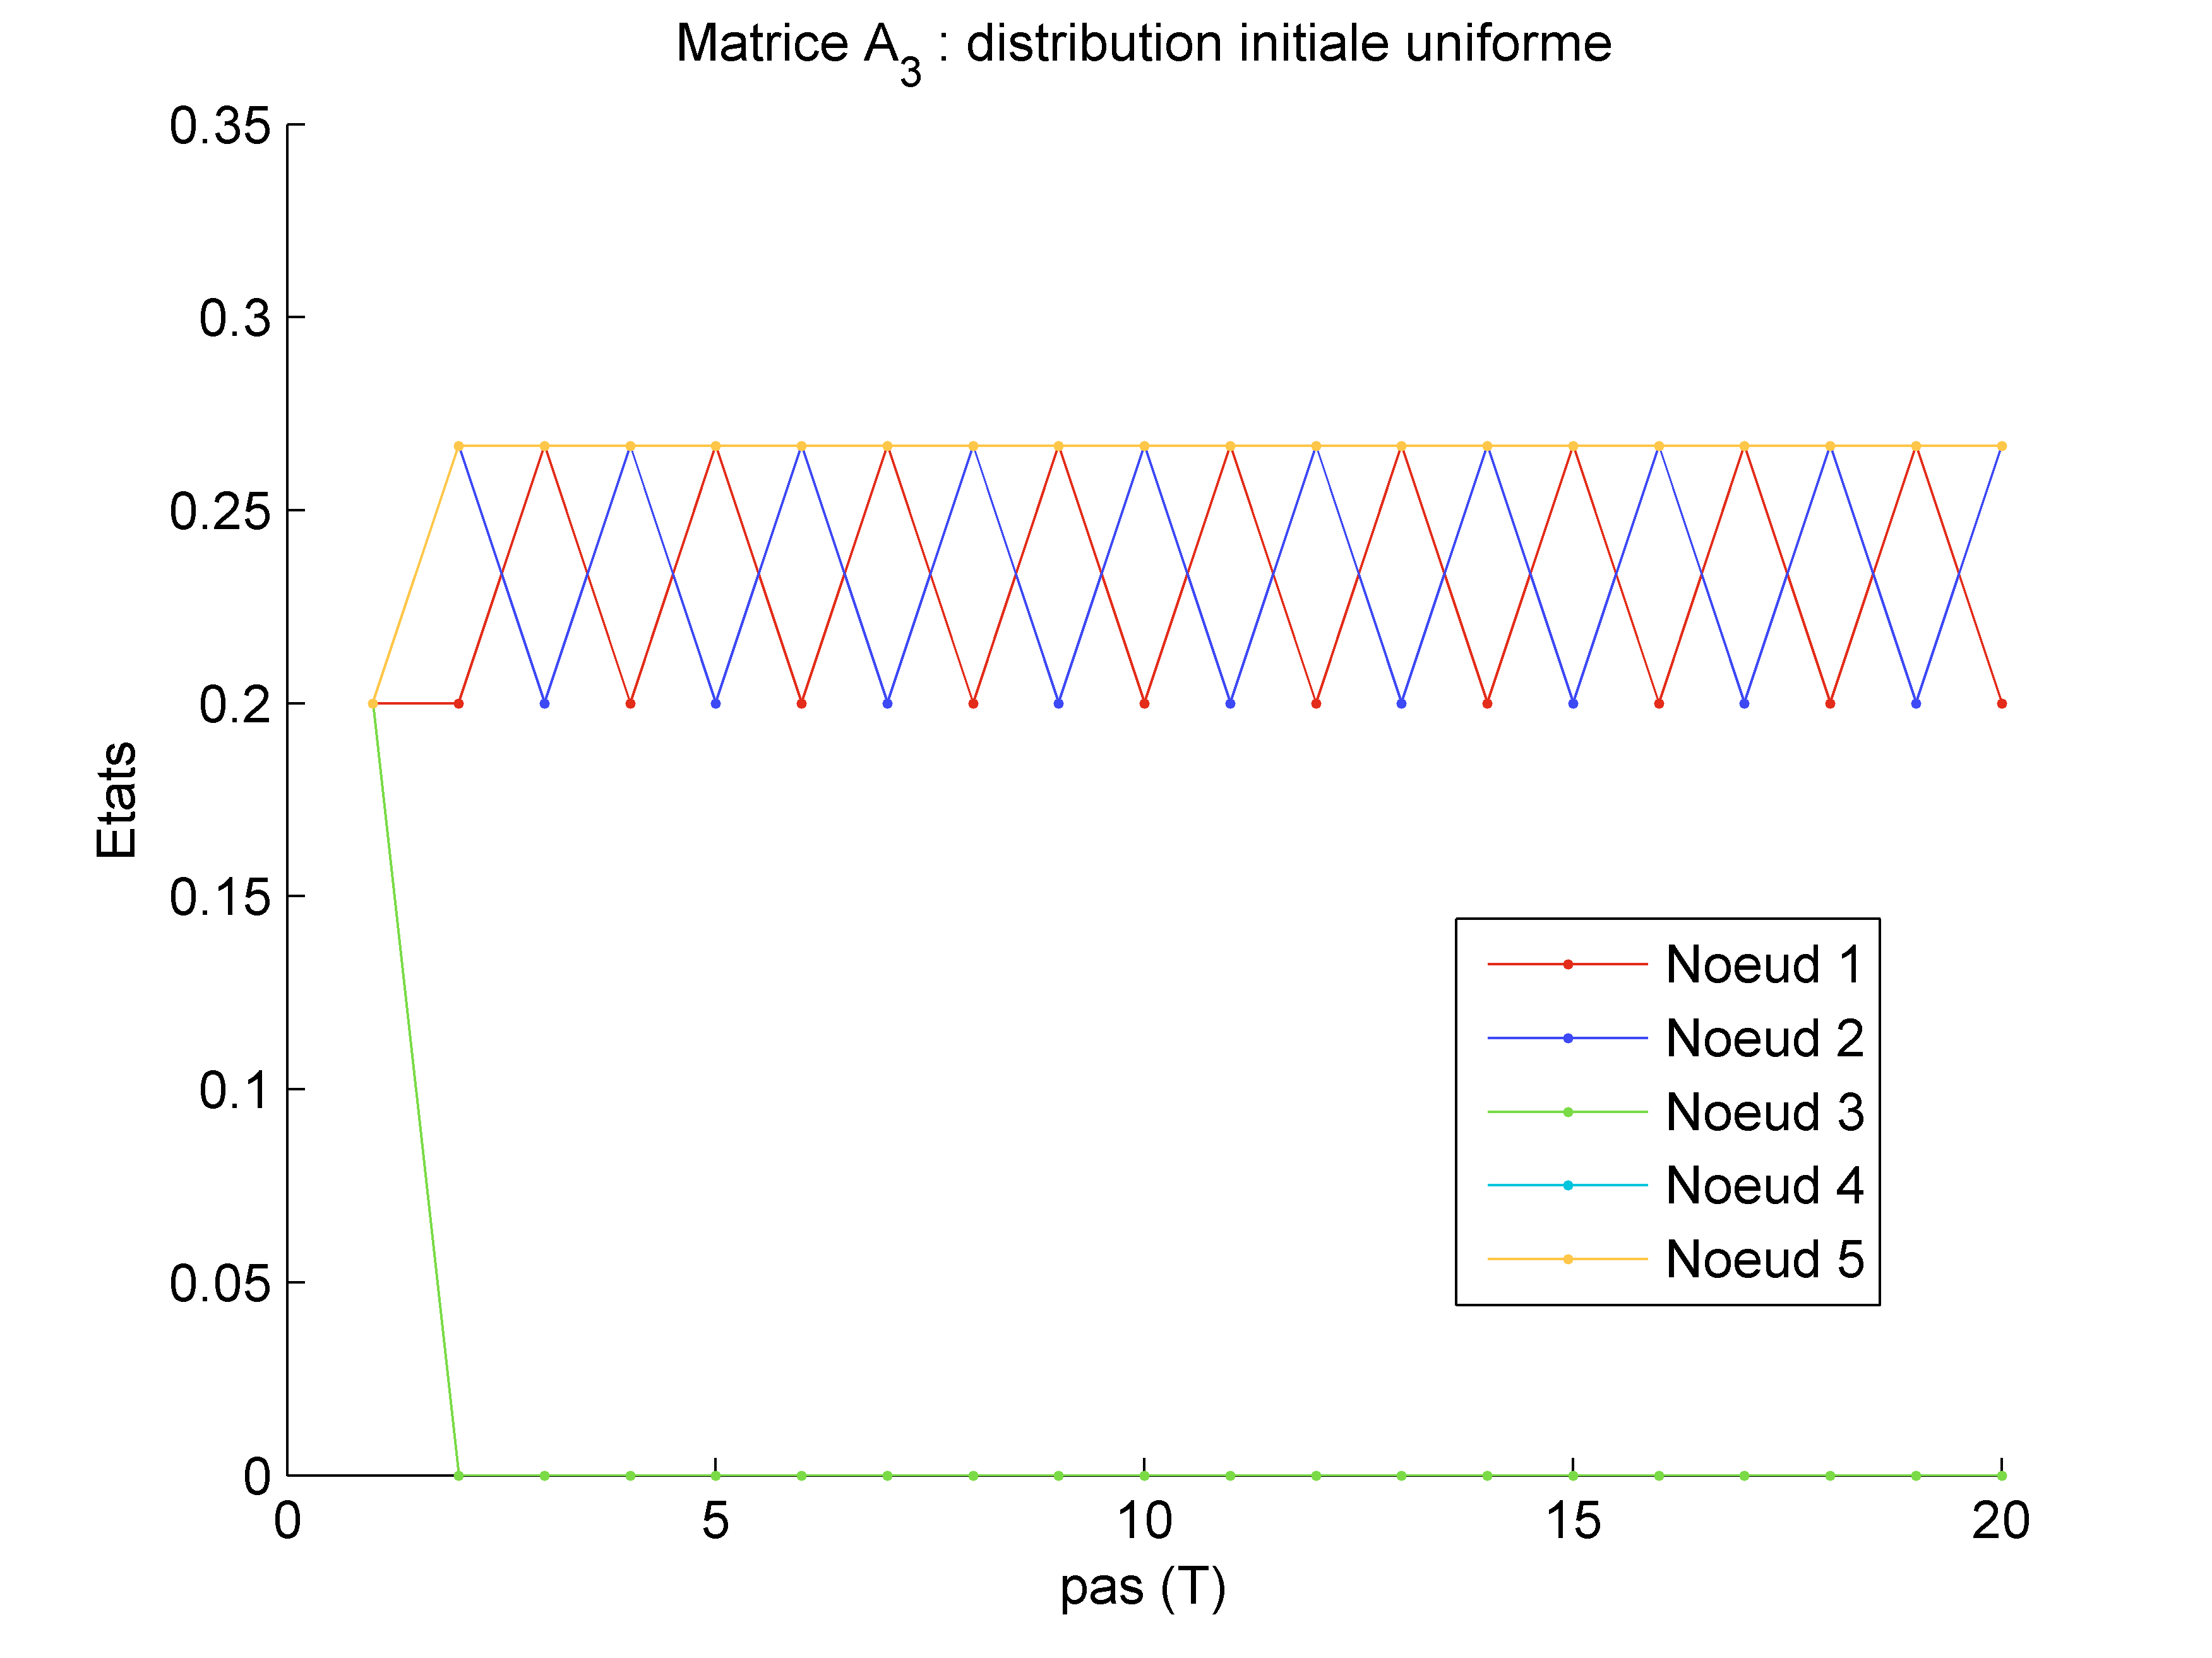
\includegraphics[scale=0.45]{../images/q118_evol_31.png}\label{sfig:q118_evol}}
	\subfigure[Depuis le noeud 1]{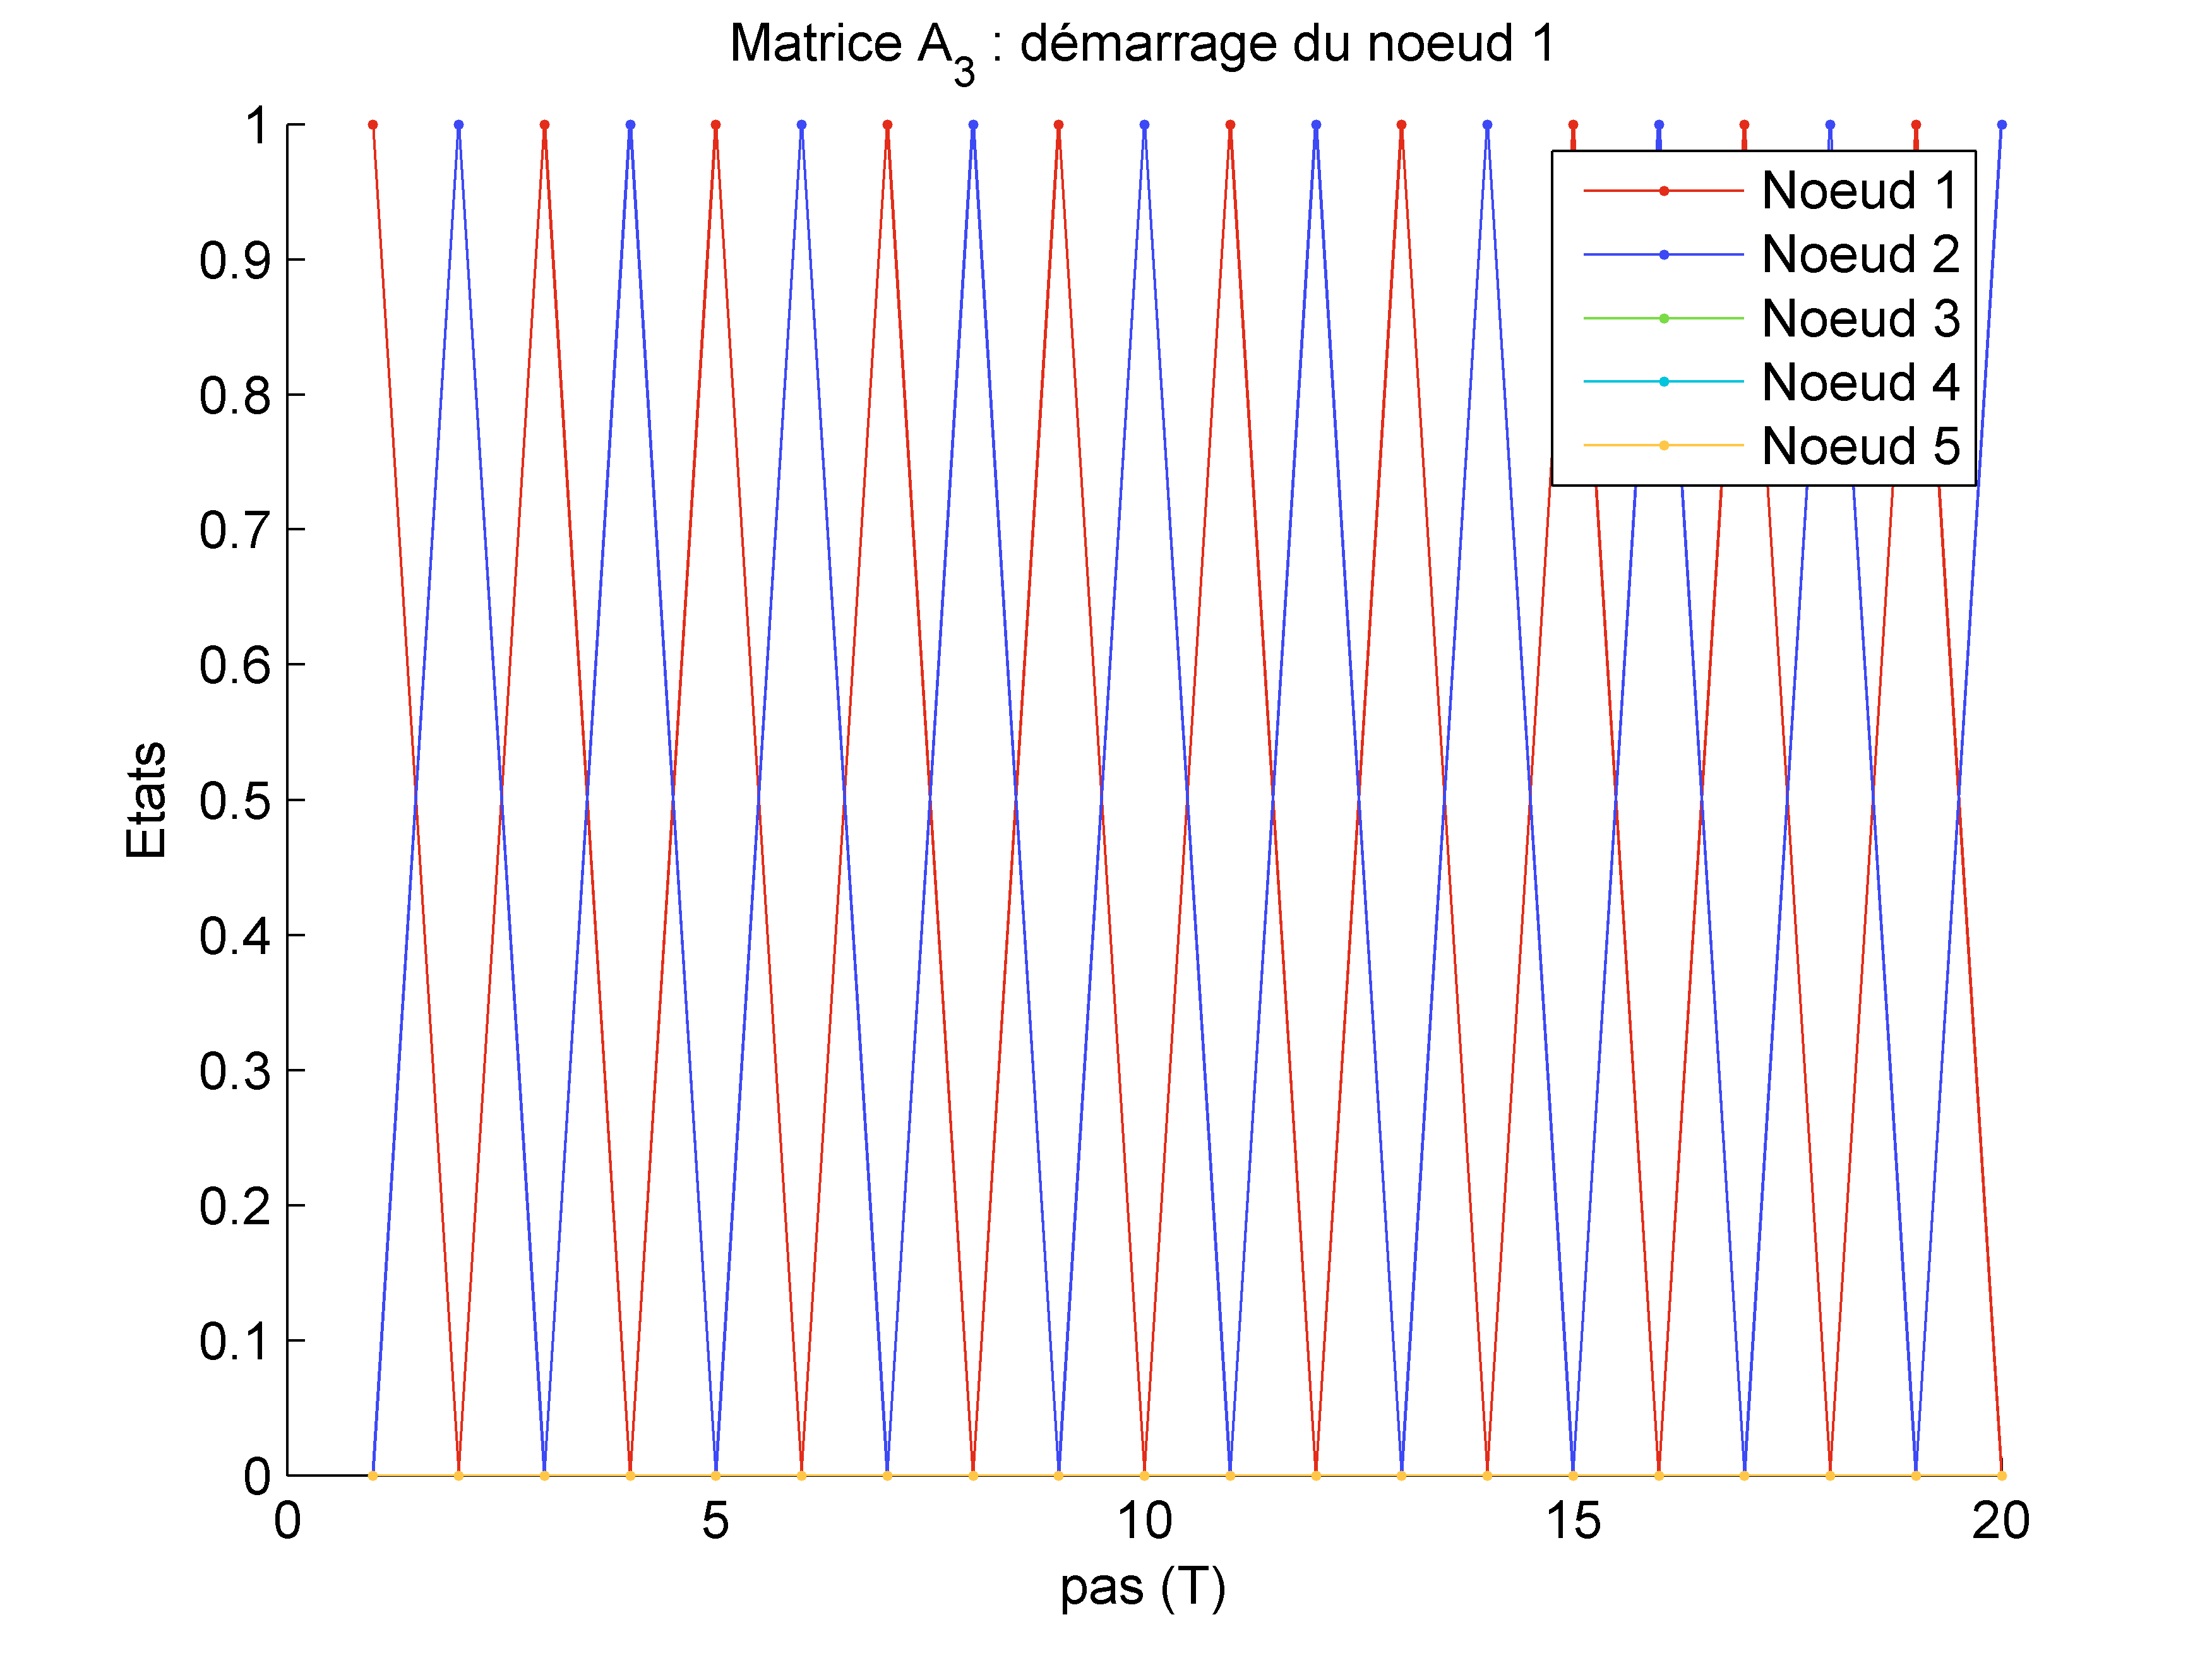
\includegraphics[scale=0.45]{../images/q118_evol_32.png}\label{sfig:q118_evol}}
	\caption{Évolution des distributions de probabilités}
	\label{fig:q118}
\end{figure}
\paragraph{2)} 
\section{Téléportation}
\paragraph{1)}
La formule utilisée pour calculer la matrice de transition $Q_t$ du modèle du surfeur avec téléportation est la suivante :
\[
	Q_t = (1 - \alpha) Q' + \alpha \tilde{Q}
\]
où $Q'$ et $\tilde{Q}$ sont des matrices de transition et $\alpha$ la probabilité de téléportation. 
\paragraph{}
La première est la matrice de transition du graphe initial auquel on a rajouté des arêtes partant des \textit{dangling nodes}. Elle a été calculée en remplaçant par $\frac{1}{n}$ tous les éléments de la matrice $Q$ situés dans des lignes ne contenant que des 0. Cette valeur $\frac{1}{n}$ a été choisie en considérant une densité de probabilité uniforme entre les différentes arêtes partant des \textit{dangling nodes}. 
\paragraph{}
La seconde est la matrice de transition du graphe complet formé des noeuds du graphe initial. Autrement dit, la matrice de transition représentant la téléportation. Une combinaison linéaire de paramètre $\alpha$ est ensuite appliquée aux deux matrices pour trouver la matrice $Q_t$.
\paragraph{2)}
Pour que la distribution stationnaire $\pi_s$ soit unique, \textbf{il faut que la chaîne de Markov soit irréductible}. Autrement dit, il faut que pour tout couple de nœuds $(i_1$, $i_2)$, il existe une arête les reliant (un probabilité non-nulle de passer de $i_1$ à $i_2$). Cette propriété est vérifiée avec le modèle du surfeur modifié puisque la téléportation permet, depuis tout noeud, de se diriger vers un autre noeud tant que $\alpha > 0$. 
\paragraph{}
A partir du moment où $\alpha = 0$, on est plus assuré que chaque paire de nœuds est reliée par une arête et donc que $\pi_s$ est bien stationnaire.
\paragraph{3)} 
Le classement des sites les plus visités, obtenus à l'aide de la distribution stationnaire, est donné dans la Table \ref{tab:best_page_rank}.
\begin{table}[h]
	\center
	\begin{tabular}{|c|c|c|}
		\hline
		N\degre & PageRank & Page \\
		\hline
		1 & 0.0045 & http://purl.org/rss/1.0/modules/content \\
		2 & 0.0027 & http://www.ulg.ac.be \\
		3 & 0.0024 & http://ogp.me/ns$\sharp$ \\
		4 & 0.0024 & http://www.gre-liege.be  \\
		5 & 0.0023 & http://blog.intelliterwal.net  \\
		6 & 0.0023 & http://www.jalios.com  \\
		7 & 0.0022 & http://www.vmfnet.be  \\
		8 & 0.0022 & http://www.alinoa.be  \\
		9 & 0.0022 & http://www.ulb.ac.be  \\
		10 & 0.0022 & http://www.cedia.ulg.ac.be  \\
		\hline
	\end{tabular}
	\caption{Classement des sites ayant le meilleur PageRank ($\alpha = 0.15$)}
	\label{tab:best_page_rank}
\end{table}
\paragraph{4)}
Soit$ X_{t_j}$ la variable aléatoire qui prend la valeur $p_i$ au temps $t_j$ si le surfeur est sur la page i.
On veut calculer : $$
P(X_{t_2} = p_2 | X_{t_3} = p_3 , X_{t_1} = p_1)
$$
En appliquant la formule de Bayes et en se rappelant de la propriété d'une chaîne de Markov, on obtient :
$$ \dfrac{P(X_{t_2} = p_2 | X_{t_1} = p_1) \cdot P(X_{t_3} = p_3 | X_{t_2} = p_2,)}{P(X_{t_3} = p_3 | X_{t_1} = p_1)} $$

Lorsque l'on passe à la notation matricielle, on a :

$$\dfrac{Q^{t_3 - t_2}(p_3, p_2) \cdot Q^{t_2 - t_1}(p_2, p_1)}{Q^{t_3 - t_1}(p_3, p_1)}
$$

Enfin en appliquant la formule pour le cas désigné dans l'énoncé, nous obtenons :

$$\dfrac{Q^{10}(p_3, p_2) \cdot Q^{9}(p_2, p_1)}{Q^{19}(p_3, p_1)} = 0.0308
$$

\section{Effet de $\alpha$}
\label{sec:effet_alpha}
\paragraph{1)}
Pour prouver que le score PageRank de toute page est au moins $\frac{\alpha}{n}$ ($n$ est le nombre de pages), on peut développer une expression "\textit{explicite}" des éléments de la matrice $Q_t$ en utilisant la formule donnée précédemment : 
\[
Q_t(i,j) = q_{ij} (1 - \alpha) + \dfrac{1}{n}\alpha\\
\]
où $q_{ij}$ est un élément de la matrice $Q'$. Connaissant la relation qui lie $\pi^{(k)}$ et $\pi^{(k-1)}$, on a :
\[
\begin{aligned}
\pi^{(k)}_j &= \sum\limits_{i = 1}^n Q_t(i,j)\pi^{(k-1)}_i\\
 &= \sum\limits_{i = 1}^n \left(q_{ij} (1 - \alpha) + \dfrac{\alpha}{n}\right)\pi^{(k-1)}_i\\
 &= \sum\limits_{i = 1}^n q_{ij} (1 - \alpha) \pi^{(k-1)}_i + \sum\limits_{i = 1}^n \dfrac{\alpha}{n} \pi^{(k-1)}_i\\
 &= \dfrac{\alpha}{n} + \underbrace{(1 - \alpha) \sum\limits_{i = 1}^n q_{ij} \pi^{(k-1)}_i}_{> 0}
\end{aligned}
\]
Le deuxième terme est inférieur à 1 (et même inférieur à $(1 - \frac{\alpha}{n})$ afin de respecter le deuxième axiome de Kolmogorov) et surtout, positif. De ce fait, on peut affirmer que :
\[
\pi^{(k)}_j \geq \dfrac{\alpha}{n}
\]
On peut interpréter le cas où $\alpha = 0$ comme le cas où il n'y a pas de téléportation et le cas où $\alpha = 1$ comme le cas où il n'y a que téléportation (le surfeur n'utilise plus les liens). Remarquons les valeurs prises par les distributions dans les deux cas :
\[
\begin{array}{l}
\pi_{\alpha = 0}^{(k)} = \pi^{(k-1)} Q'\\ \\
\pi_{j,\alpha = 1}^{(k)} = \frac{1}{n}, \forall j
\end{array}
\]
\paragraph{}
Dans le deuxième cas, les PageRank de toutes les pages seront égaux et vaudront $\frac{1}{n}$. Afin de vérifier cette affirmation, nous avons calculé la distribution stationnaire pour un $\alpha = 1$ et l'avons mise en parallèle avec la distribution stationnaire pour $\alpha = 0.15$. Le résultat est édifiant (voir Table \ref{tab:alpha_comp}, on constate en effet un PageRank uniforme dans le cas où $\alpha = 1$ .
\begin{table}[h]
	\center
	\begin{tabular}{|c|c|c|}
		\hline 
		$\alpha$   & 0.15  & 1 \\
		\hline
	 	Moyenne    & 0.002 & 0.002\\
	 	Ecart-type & 1.3000e-04 & \textbf{4.7753e-18} \\
	 	Min.       & 0.0019 & 0.002\\
	 	Max.       & 0.0045 & 0.002\\
	 	\hline
	\end{tabular}
	\caption{Statistiques à propos des distributions stationnaires avec $\alpha = 0.15$ et $\alpha = 1$}
	\label{tab:alpha_comp}
\end{table}
\paragraph{2)}
Nous avons analysé l'évolution du PageRank de certaines pages lorsque alpha évolue. En regardant la Figure \ref{sfig:evolPagerank} , on observe que plus alpha est grand, plus le PageRank des pages tend à s'uniformiser. En effet, un PageRank élevé au départ va diminuer avec l'augmentation de $\alpha$, tandis qu'un PageRank assez bas va augmenter avec $\alpha$ vu que plus alpha est élevé, plus la probabilité d'arriver sur une telle page s'uniformise.   


\begin{figure}[h]
	\center
	\subfigure{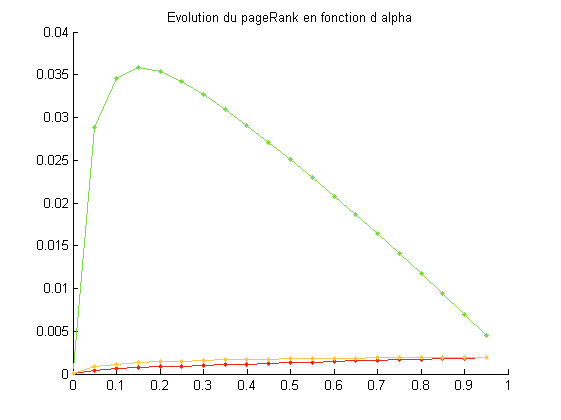
\includegraphics[scale=0.45]{../images/evolPagerank.png}\label{sfig:evolPageRankAlpha}}
	\subfigure{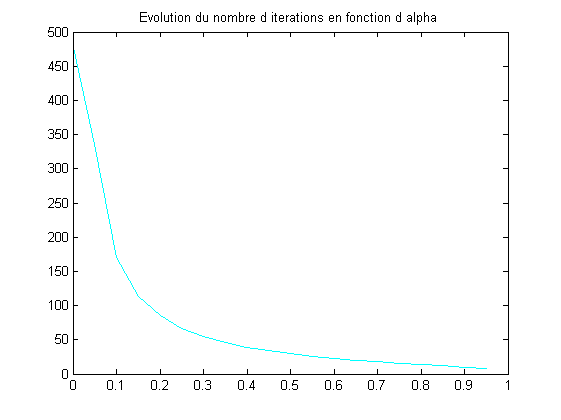
\includegraphics[scale=0.45]{../images/nbItAlpha.png}\label{sfig:nbItAlph}}
	\caption{Évolution du PageRank et du nombre d'itérations avec $\alpha$}
\end{figure}
\paragraph{3)}
Nous avons déterminé l'évolution du nombre d'itérations nécessaires pour trouver une distribution stationnaire lorsque $\alpha$ varie. Les résultats sont présentés sur la Figure \ref{sfig:nbItAlpha} :  

Les résultats observés sont attendus car il est logique de trouver une distribution stationnaire très rapidement lorsque $\alpha$ tend vers 1, étant donné que on ne tient compte que de la téléportation: la probabilité d'arriver sur une page ou une autre partant d'une page donnée est uniforme. Dans le cas contraire, lorsque alpha tend vers zéro, on repose plus sur le graphe de départ ce qui est plus compliqué à calculer qu'une répartition uniforme.
\chapter{Question 2}
\section{Estimation d'une matrice de transition}
\subsection{Méthode d'estimation}
Avant tout, voici les quelques notations que nous utiliserons : 
\begin{itemize}
	\item $n$, le nombre de noeuds dans le graphe
	\item $X$, la trace fournie (chaîne de Markov)
	\item $Q_{est}$, la matrice de transition recherchée
	\[
		Q_{est} = 
		\begin{pmatrix}
			\theta_{11} & \cdots & \theta_{1n}\\
			\vdots & \ddots & \vdots\\
			\theta_{n1} & \cdots & \theta_{nn}\\
		\end{pmatrix}
	\]
	\item $N$, la matrice dont l'élément $\beta_{ij}$ est le nombre de transition de l'état $i$ à $j$ dans la trace $X$
	\item $\sigma_i$, la somme de la $i^{\text{ème}}$ ligne de la matrice $N$
	\item $\underline{\theta}_i$; le vecteur contenant les probabilités pour passer du nœud $i$ à un autre nœud : 
	\[
		\underline{\theta}_i = [\theta_{i1} \cdots \theta_{in}]
	\]
	\item $P(X|\underline{\theta}_i)$, la probabilité d'observer les départs du nœud $i$ présents dans la trace connaissant $\underline{\theta}_i$ 
	\[
		P(X|\underline{\theta}_i) = \theta_{i1}^{\beta_{i1}} \times \cdots \times \theta_{i(n - 1)}^{\beta_{i(n - 1)}} \times \left(1 - \sum\limits_{k = 1}^{n - 1} \theta_{ik}\right)^{\beta_{in}} = \left(1 - \sum\limits_{k = 1}^{n - 1} \theta_{ik}\right)^{\beta_{in}} \times \prod\limits_{k = 1}^{n - 1} \theta_{ik}^{\beta_{ik}}
	\]
	\item $S_i$, le système de $n - 1$ équations à résoudre pour trouver la ligne $i$ de la matrice de transition par la méthode du maximum de vraisemblance. On note $S_{ij}$ la $j^{\text{ième}}$ équation de ce système.
	\[
		S_i \equiv 
		\left\{
		\begin{array}{c}
		\dfrac{\partial P(X|\underline{\theta}_i)}{\partial \theta_{i1}} = 0\\
		\vdots\\
		\dfrac{\partial P(X|\underline{\theta}_i)}{\partial \theta_{i(n-1)}} = 0\\
		\end{array}
		\right.
	\] 
	La résolution de ce système ne donne que les $n-1$ probabilités de la ligne $i$. Il suffit de les sommer pour obtenir la $n^{\text{ième}}$.
\end{itemize}
\paragraph{}
Développons l'équation trouvée ci-dessus (pour $j \in [2, n-2]$ mais que l'on peut facilement généraliser pour les cas où $j = 1$ ou $(n-1)$):

\[
	\begin{aligned}
		S_{ij} &= \left[\beta_{ij} \theta_{ij}^{\beta_{ij} - 1} \left(1 - \sum\limits_{k = 1}^{n - 1} \theta_{ik}\right)^{\beta_{in}} - \beta_{in} \left(1 - \sum\limits_{k = 1}^{n - 1} \theta_{ik}\right)^{\beta_{in} - 1} \theta_{ij}^{\beta_{ij}}\right] \times \prod\limits_{k = 1, k \neq j}^{n - 1} \theta_{ik}^{\beta_{ik}}\\
		&= \left[\beta_{ij}  \left(1 - \sum\limits_{k = 1}^{n - 1} \theta_{ik}\right) - \beta_{in}  \theta_{ij}\right]\times \left(1 - \sum\limits_{k = 1}^{n - 1} \theta_{ik}\right)^{\beta_{in} - 1} \times \theta_{ij}^{\beta_{ij} - 1} \times \prod\limits_{k = 1, k \neq j}^{n - 1} \theta_{ik}^{\beta_{ik}} = 0\\
	\end{aligned}
\]
Il nous reste à résoudre l'équation suivante :
\[
	\begin{aligned}
		&\beta_{ij} \left(1 - \sum\limits_{k = 1}^{n - 1} \theta_{ik}\right) - \beta_{in} \theta_{ij} = 0\\
		\Leftrightarrow \text{ }&\beta_{ij} \left(1 - \sum\limits_{k = 1}^{n - 1} \theta_{ik}\right) = \beta_{in} \theta_{ij}\\
		\Leftrightarrow \text{ }& \dfrac{\beta_{in}}{\beta_{ij}} \theta_{ij} + \sum\limits_{k = 1}^{n - 1} \theta_{ik} = 1\\
		\Leftrightarrow \text{ }& \left(\dfrac{\beta_{in}}{\beta_{ij}} + 1\right) \theta_{ij} + \sum\limits_{k = 1, k \neq j}^{n - 1} \theta_{ik} = 1 \text{ } (1)	
	\end{aligned}
\]
Le système $S_i$ peut se réécrire sous forme matricielle de la manière suivante : 
\[
S_i \equiv 
\begin{pmatrix}
\left(\dfrac{\beta_{in} + \beta_{i1}}{\beta_{i1}}\right) & 1 & \cdots & 1 \\
1 & \ddots &  \ddots & \vdots \\
\vdots &  \ddots & \ddots & 1\\
1 & \cdots & 1   & \left(\dfrac{\beta_{in} + \beta_{i(n - 1)}}{\beta_{i(n - 1)}}\right)
\end{pmatrix}
\begin{pmatrix}
\theta_{i1}\\
\vdots\\
\theta_{i(n - 1)}
\end{pmatrix}
= 
\begin{pmatrix}
1\\
\vdots\\
1\\
\end{pmatrix}
\]
La résolution de ce système pour chaque ligne permet d'obtenir une estimation de la matrice de transition. Néanmoins, cette méthode est extrêmement inefficace puisqu'elle nécessite $n$ résolutions du système (la résolution d'un système étant elle-même une opération coûteuse en terme de temps de calcul). Bien qu'à notre échelle ($n = 50$), cette complexité élevée ne soit pas gênante, une simplification de la méthode d'estimation serait tout de même bienvenue. Repartons de l'équation $(1)$ : 
\[
\begin{aligned}
	&\left(\dfrac{\beta_{in}}{\beta_{ij}} + 1\right) \theta_{ij} + \sum\limits_{k = 1, k \neq j}^{n - 1} \theta_{ik} = 1\\
	&\Leftrightarrow \dfrac{\beta_{in}}{\beta_{ij}} \theta_{ij} + \theta_{ij} = 1 - \sum\limits_{k = 1, k \neq j}^{n - 1} \theta_{ik}\\
	&\Leftrightarrow \dfrac{\beta_{in}}{\beta_{ij}} \theta_{ij} + \theta_{ij} = \theta_{ij} + \theta_{in}\\
	&\Leftrightarrow \theta_{ij}= \dfrac{\theta_{in}}{\beta_{in}} \beta_{ij}\text{ }(2)\\
	&\Leftrightarrow \sum\limits_{i = 0}^{n - 1} \theta_{ij} = \dfrac{\theta_{in}}{\beta_{in}} \sum\limits_{i = 0}^{n - 1}\beta_{ij}\\
	&\Leftrightarrow 1 - \theta_{in} = \dfrac{\theta_{in}}{\beta_{in}} \left(\sigma_i - \beta_{in}\right)\\	
	&\Leftrightarrow \theta_{in} = \dfrac{\beta_{in}}{\sigma_{i}} \text{ }(3)\\	
\end{aligned}
\]
\paragraph{}
En injectant l'équation $(3)$ dans l'équation $(2)$, on obtient l'équation :
\[
\theta_{ij} = \dfrac{\beta_{ij}}{\sigma_{i}}
\]
\paragraph{}
La formule ci-dessus nous permet de simplifier l'estimation puisque qu'il suffit maintenant de \textbf{diviser chaque élément $\beta_{ij}
$ de la matrice $N$ par la somme de la ligne dans laquelle il se trouve} pour trouver la matrice de transition. Il ne reste plus qu'à régler le problème où
\[
\beta_{ij} = 0, \forall j \in [1,n]
\]
En effet, cette situation mènerait à une division par zéro. Il faut donc appliquer un traitement à la matrice $N$ afin de supprimer les valeurs nulles.
\subsubsection{Smoothing}
Plusieurs techniques de lissage existent dont la méthode de Laplace (\textit{Laplace smoothing}) qui consiste à ajouter 1 à tous les éléments comptés.

\subsection{Utilisation des modèles estimés}
\label{ssec:util_esti}
Une méthode pour déterminer l'origine des traces d'un ensemble de traces consiste à calculer la probabilité $P(Q_i|tr_k)$ que $tr_k$ provienne d'une certaine matrice de transition $Q_i$ (la matrice de transition définissant le comportement d'un surfeur). Il suffira ensuite de prendre le surfeur dont la matrice de transition mène à la plus grande probabilité. Autrement dit : 
\[
arg \max\limits_i P(Q_i|tr_k)
\]
A l'aide de la formule de Bayes, on peut développer : 
\[
P(Q_i|tr_k) = \dfrac{P(tr_k|Q_i) P(Q_i)}{\sum\limits_{j = 1}^n P(tr_k|Q_j) P(Q_j)}
\]
où le terme $P(tr_k|Q_i)$ est la vraisemblance de la trace connaissant la matrice $Q_i$ et $P(Q_i)$ est la probabilité qu'une trace provienne du surfeur $i$.
\paragraph{}
Dans notre cas, la vraisemblance est un nombre tellement petit qu'il n'est pas représentable sur un ordinateur (à moins d'utiliser des bibliothèques spéciales). Nous avons donc décidé d'utiliser la \textbf{log-vraisemblance} de sorte que les nombres soient manipulables. 
\paragraph{} 
Étant donné que les traces $tr_k$ ne peuvent appartenir qu'à deux surfeurs, nous pouvons aussi modifier notre règle de décision. Pour ce faire, nous définissons :
\[
\begin{aligned}
r &= \log \dfrac{P(Q_1|tr_k)}{P(Q_2|tr_k)}\\
&= \log \dfrac{P(tr_k|Q_1) P(Q_1)}{P(tr_k|Q_2) P(Q_2)}\\
&= \log P(tr_k|Q_1) - \log P(tr_k|Q_2) + \log \dfrac{P(Q_1)}{P(Q_2)}
\end{aligned}
\]
Si $r > 0$ alors la trace d'origine provient du \textbf{surfer 1} sinon elle provient du \textbf{surfer 2}. Notons que dans notre cas :
\[ 
	P(Q_i) = \frac{1}{2}, \forall i \in [1,2]
\]
En effet, nous savons que parmi les 20 traces à évaluer, 10 appartiennent au premier (soit la moitié) et 10 au deuxième (soit l'autre moitié).  
\subsubsection{Calcul de la vraisemblance}
Pour une trace $X$, une matrice $N$ contenant les éléments $\beta_{ij}$ (nombre de transition de l'état $i$ à $j$ dans $X$) et une matrice de transition $Q$, la vraisemblance est donnée par : 
\[
P(X|Q) = \prod\limits_{i = 1}^n \prod\limits_{j = 1}^n \theta_{ij}^{\beta_{ij}}
\]
Comme expliqué plus haut, nous utiliserons la log-vraisemblance qui se calcule comme suit :
\[
log P(X|Q) = \sum\limits_{i = 1}^n\sum\limits_{i = 1}^n \beta_{ij} \log \theta_{ij}
\]

\subsection{Analyse des 20 traces}
En appliquant la méthode expliquée dans la Section \ref{ssec:util_esti}, nous avons obtenu les résultats donnés dans la Table \ref{tab:surf_trace}. Nous ne savons pas calculer explicitement la probabilité $ P(Q_i|tr_k)$. En effet, nous ne savons calculer que le $log( P(tr_k|Q_i) )$ vu que les valeurs sont très petites or, le dénominateur développé plus haut fait la somme des probabilités  $ P(Q_i|tr)$.  
\begin{table}[ht]
	\center
	\begin{tabular}{|c|cc|}
		\hline
		Trace & $r$ & Provient de \\
		\hline
		1 & $ -0.4361$ & $\mathbf{2}$ \\
		2 & $57.737$ & $\mathbf{1}$ \\
		3 & $70.562$ & $\mathbf{1}$ \\
		4 & $68.022$ & $\mathbf{1}$ \\
		5 & $-153.35$ & $\mathbf{2}$ \\
		6 & $127.45$ & $\mathbf{1}$ \\
		7 & $-47.847$ & $\mathbf{2}$ \\
		8 & $47.912$ & $\mathbf{1}$ \\
		9 & $-13.472$ & $\mathbf{2}$ \\
		10 & $-10.209$ & $\mathbf{2}$ \\
		11 & $-183.48$ & $\mathbf{2}$ \\
		12 & $-155.67$ & $\mathbf{2}$ \\
		13 & $52.513$ & $\mathbf{1}$ \\
		14 & $10.682$ & $\mathbf{1}$ \\
		15 & $19.723$ & $\mathbf{1}$ \\
		16 & $-104.7$ & $\mathbf{2}$ \\
		17 & $-34.937$ & $\mathbf{2}$ \\
		18 & $12.536$ & $\mathbf{1}$ \\
		19 & $-53.645$ & $\mathbf{2}$ \\
		20 & $126.89$ & $\mathbf{1}$ \\
		\hline
	\end{tabular}
	\caption{Recherche des surfeur ayant engendré les traces}
	\label{tab:surf_trace}
\end{table}
\subsection{Hypothèses, fiabilité et limites}
Pour appliquer la méthode du maximum de vraisemblance, on doit uniquement connaitre les probabilités qui nous sont données par le graphe. Nous avons testé les résultats de notre méthode: 

\subsubsection{Test de la méthode}
Pour tester cette méthode, nous avons procédé en plusieurs étapes : 
\begin{itemize}
	\item Définition d'une matrice d'adjacence $A$ de taille $k \times k$ (i, $k = 5$)
	\item Calcul de la matrice de transition $Q$ et génération de $n$ (ici, $n = 50$) chaîne de Markov $X_i$ de taille $m$ (ici, $m = 1000$)
	\item Génération de $n$ estimations $Q_{est,i}$ de la matrice de transition sur base des chaînes générées
	\item Calcul de l'erreur quadratique moyenne $E$ (EQM) pour chaque $\theta_{ij}$ 
\end{itemize}
\paragraph{}
En utilisant cette méthode nous avons obtenu des résultats intéressants. Ci-dessous sont données la matrice $Q$ exacte, l'erreur quadratique moyenne sur les $50$ générations et $Q_{est}$, une des matrices estimées :
\[
Q = 
\begin{pmatrix}
0.1000 & 0.3500 & 0.3500 & 0.1000 & 0.1000\\
0.1000 & 0.1000 & 0.1000 & 0.6000 & 0.1000\\
0.3500 & 0.3500 & 0.1000 & 0.1000 & 0.1000\\
0.1000 & 0.1000 & 0.3500 & 0.1000 & 0.3500\\
0.3500 & 0.1000 & 0.1000 & 0.3500 & 0.1000\\
\end{pmatrix}
\]
\[
E = 
\begin{pmatrix}
0.0006 & 0.0008 & 0.0015 & 0.0005 & 0.0003\\
0.0005 & 0.0003 & 0.0005 & 0.0008 & 0.0003\\
0.0012 & 0.0009 & 0.0004 & 0.0005 & 0.0005\\
0.0004 & 0.0002 & 0.0009 & 0.0004 & 0.0012\\
0.0017 & 0.0006 & 0.0004 & 0.0016 & 0.0004\\
\end{pmatrix}
\]
\[
Q_{est} = 
\begin{pmatrix}
0.0883 & 0.3282 & 0.3659 & 0.0952 & 0.1224\\
0.1075 & 0.1061 & 0.1016 & 0.5906 & 0.0942\\
0.3312 & 0.3629 & 0.1060 & 0.0906 & 0.1093\\
0.0946 & 0.1123 & 0.3322 & 0.1064 & 0.3546\\
0.3529 & 0.0997 & 0.1124 & 0.3390 & 0.0960\\
\end{pmatrix}
\]
Nous avons calculé la moyenne des erreurs quadratiques contenues dans $E$ et avons trouvé une erreur moyenne d'environ $5\%$ pour cette configuration. La Table \ref{tab:eqm_m} contient l'évolution de cette grandeur lorsque $m$ varie. On constate (et c'était attendu) que l'erreur quadratique diminue au fur et à mesure que la taille des chaînes de Markov utilisées augmente. 
\paragraph{}
On peut conclure que la taille des traces relativement courte permettent d'obtenir une erreur quadratique tout à fait acceptable.
\paragraph{} 
Afin de pouvoir mettre le problème à l'échelle, il est plus intéressant d'étudier le paramètre $\frac{m}{k}$. En effet, plus ce paramètre est petit, moins la chaîne de Markov aura tendance à être représentative de la matrice de transition et inversément. Dans notre cas, nous obtenons un rapport $\frac{m}{k} = 20$ qui donne déjà une bonne précision.
\begin{table}[ht]
	\center
	\begin{tabular}{|c||c|c|}
		\hline
		$m$ & \textbf{Moyenne de l'erreur} & $\frac{m}{k}$\\
		\hline
		$100$ & $0.0075$ & 20\\
		$\mathbf{1000}$ & $\mathbf{\num{6.9755e-04}}$ & 200\\
		$5000$ & $\num{1.5653e-04}$ & 1000\\
		$10000$ & $\num{7.2594e-05}$ & 2000\\
		\hline
	\end{tabular}
	\caption{Erreur moyenne en fonction du paramètre $m$}
	\label{tab:eqm_m}
\end{table}
\subsection{Applications possibles de la méthode}
Les chaînes de Markov ont de nombreuses applications possibles dans des domaines très variés tels que les sciences sociales, la biologie, les sciences économiques et pleins d'autres. \\ \\

Pour citer quelques exemples, on utilise les modèles de Markov pour identifier les régions de l'ADN génomique qui codent les gènes, pour la reconnaissance et la synthèse vocale, pour prédire les éruptions d'un geyser et bien d'autres encore. \\ \\

 Dans notre parcours universitaire, nous avons déjà utilisé un modèle de Markov caché pour définir une caractéristique d'un texte (langue, auteur). L'algorithme se basait sur plusieurs échantillons de textes ayant des caractéristiques différentes. Nous établissions des modèles sur base de ces échantillons et testions ensuite l'appartenance d'un texte à l'un des modèles. Grâce à cet algorithme, nous avons pu discerner la langue d'un texte, le langage d'un code, l'auteur d'un livre à partir d'échantillons pour chaque caractéristique. Malgré la simplicité de ce programme, nous pouvions déjà faire un certain nombre de tests différents. 

\section{Estimation de $\alpha$}
\paragraph{1)} Le paramètre $\alpha$ est un paramètre de la matrice de transition représentant un surfeur aléatoire. Nous avons défini dans la Section \ref{sec:effet_alpha}, la formule définissant chaque élément de cette matrice de transiton en fonction de $\alpha$ pour le modèle du surfeur aléatoire : 
\[
Q_t(i,j) = q_{ij} (1 - \alpha) + \dfrac{\alpha}{n}\\
\]
Un première approche est d'utiliser cette formule afin de définir le paramètre recherché. 
\paragraph{}
La seule inconnue du membre de droite est $\alpha$. En effet, nous connaissons de manière exacte le terme $q_{ij}$ puisque nous connaissons le graphe sur lequel le surfeur se déplace. En ce qui concerne le membre de gauche, nous sommes capable de l'estimer par la méthode développée au point précédent. Il est important de garder en tête que \textbf{cette matrice de transition est estimée} et que chaque probabilité de la matrice est entachée d'une erreur qui se propagera, lors de la résolution, dans la valeur de $\alpha$. 
\paragraph{}
Nous avons à notre disposition $n^2$ équations qui vont toutes nous donner des valeurs différentes pour $\alpha$. 
\end{document}
